% Seminar 11: Fractal markets hypothesis and long memory
% Statistics of Financial Markets -- Bachelor's programme, Bucharest University of Economic Studies
% GENERATED by latex/build_seminar11.py -- edit the generator, not this file.
% Student version by default; the instructor version is the *_solutions.tex wrapper.
\makeatletter\@ifundefined{ifsolutions}{\expandafter\newif\csname ifsolutions\endcsname}{}\makeatother

\newcommand{\coursename}{Statistics of Financial Markets}
% Preambul comun SFM -- Statistica piețelor financiare / Statistics of Financial Markets (Beamer, 16:9)
% Același design ca MFM. Înainte de % Preambul comun SFM -- Statistica piețelor financiare / Statistics of Financial Markets (Beamer, 16:9)
% Același design ca MFM. Înainte de % Preambul comun SFM -- Statistica piețelor financiare / Statistics of Financial Markets (Beamer, 16:9)
% Același design ca MFM. Înainte de \input{../../latex/preamble} se definește
%   \newcommand{\coursename}{Statistics of Financial Markets}      (EN)
%   \newcommand{\coursename}{Statistica piețelor financiare}       (RO)  și  \def\sfmlang{ro}
% Fișierele .tex se află în EN/Courses, EN/Seminars, RO/Cursuri, RO/Seminarii (două niveluri sub rădăcină).
% Deck-urile sînt generate de latex/build_chapterN.py / build_seminarN.py (vezi latex/sfm_build.py).

\documentclass[9pt, aspectratio=169, t]{beamer}
\providecommand{\coursename}{Statistics of Financial Markets}

% Ensure content fits on slides
\setbeamersize{text margin left=8mm, text margin right=8mm}

%=============================================================================
% THEME AND STYLE CONFIGURATION
%=============================================================================
\usetheme{default}
% Using default theme for clean header/footer control

% Color Palette (matching Redispatch PDF)
\definecolor{MainBlue}{RGB}{26, 58, 110}
\definecolor{AccentBlue}{RGB}{26, 58, 110}
\definecolor{IDAred}{RGB}{205, 0, 0}
\definecolor{DarkGray}{RGB}{51, 51, 51}
\definecolor{MediumGray}{RGB}{128, 128, 128}
\definecolor{LightGray}{RGB}{248, 248, 248}
\definecolor{VeryLightGray}{RGB}{235, 235, 235}
\definecolor{KeynoteGray}{RGB}{218, 218, 218}
\definecolor{SectionGray}{RGB}{120, 120, 120}
\definecolor{FooterGray}{RGB}{100, 100, 100}
\definecolor{Crimson}{RGB}{220, 53, 69}
\definecolor{Forest}{RGB}{46, 125, 50}
\definecolor{Amber}{RGB}{181, 133, 63}
\definecolor{Orange}{RGB}{230, 126, 34}
\definecolor{Purple}{RGB}{142, 68, 173}

% Gradient background (exact Keynote 315° gradient: white to RGB 218,218,218)
\setbeamertemplate{background}{%
    \begin{tikzpicture}[remember picture, overlay]
        \shade[shading=axis, shading angle=315,
        top color=white, bottom color=KeynoteGray]
        (current page.south west) rectangle (current page.north east);
    \end{tikzpicture}%
}
% Fallback solid color for compatibility
\setbeamercolor{background canvas}{bg=}

\setbeamercolor{palette primary}{bg=MainBlue, fg=white}
\setbeamercolor{palette secondary}{bg=MainBlue!85, fg=white}
\setbeamercolor{palette tertiary}{bg=MainBlue!70, fg=white}
\setbeamercolor{structure}{fg=MainBlue}
\setbeamercolor{title}{fg=IDAred}
\setbeamercolor{frametitle}{fg=IDAred, bg=}
\setbeamercolor{block title}{bg=MainBlue, fg=white}
\setbeamercolor{block body}{bg=VeryLightGray, fg=DarkGray}
\setbeamercolor{block title alerted}{bg=Crimson, fg=white}
\setbeamercolor{block body alerted}{bg=Crimson!8, fg=DarkGray}
\setbeamercolor{block title example}{bg=Forest, fg=white}
\setbeamercolor{block body example}{bg=Forest!8, fg=DarkGray}
\setbeamercolor{item}{fg=MainBlue}

% Footer colors (override Madrid theme blue)
\setbeamercolor{author in head/foot}{fg=FooterGray, bg=}
\setbeamercolor{title in head/foot}{fg=FooterGray, bg=}
\setbeamercolor{date in head/foot}{fg=FooterGray, bg=}
\setbeamercolor{section in head/foot}{fg=FooterGray, bg=}
\setbeamercolor{subsection in head/foot}{fg=FooterGray, bg=}

% Bullet styles (apply everywhere including blocks)
\setbeamertemplate{itemize item}{\color{MainBlue}$\boxdot$}
\setbeamertemplate{itemize subitem}{\color{MainBlue}$\blacktriangleright$}
\setbeamertemplate{itemize subsubitem}{\color{MainBlue}\tiny$\bullet$}
\setbeamertemplate{itemize/enumerate body begin}{\normalsize}
\setbeamertemplate{itemize/enumerate subbody begin}{\normalsize}

% Item spacing - compact style
\setlength{\leftmargini}{10pt}       % Level 1: minimal indent
\setlength{\leftmarginii}{10pt}      % Level 2: minimal additional indent
% Compact list spacing (zero extra space before/after lists in blocks)
\makeatletter
\def\@listi{\leftmargin\leftmargini \topsep 0pt \parsep 0pt \itemsep 0pt}
\def\@listii{\leftmargin\leftmarginii \topsep 0pt \parsep 0pt \itemsep 0pt}
\makeatother

\setbeamertemplate{navigation symbols}{}

%=============================================================================
% CUSTOM HEADLINE
%=============================================================================
\setbeamertemplate{headline}{%
    \vskip10pt%
    \hbox to \paperwidth{%
        \hskip0.5cm%
        {\small\color{FooterGray}\renewcommand{\hyperlink}[2]{##2}\insertsectionhead}%
        \hfill%
        \textcolor{FooterGray}{\small\insertframenumber}%
        \hskip0.5cm%
    }%
    \vskip4pt%
    {\color{FooterGray}\hrule height 0.4pt}%
}

%=============================================================================
% CUSTOM FOOTER
%=============================================================================
\usepackage{fontawesome5}

\setbeamertemplate{footline}{%
    {\color{FooterGray}\hrule height 0.4pt}%
    \vskip4pt%
    \hbox to \paperwidth{%
        \hskip0.5cm%
        \textcolor{FooterGray}{\small\coursename}%
        \hfill%
        \raisebox{-0.1em}{%
            \begin{tikzpicture}[x=0.08em, y=0.08em, line width=0.4pt]
                \draw[FooterGray] (0,3) -- (1,4) -- (2,3.5) -- (3,5) -- (4,4) -- (5,6) -- (6,5.5) -- (7,4) -- (8,5) -- (9,7) -- (10,6) -- (11,5) -- (12,6.5) -- (13,8) -- (14,7) -- (15,6) -- (16,7.5) -- (17,9) -- (18,8) -- (19,7) -- (20,8.5) -- (21,10) -- (22,9) -- (23,8) -- (24,9.5);
            \end{tikzpicture}%
        }%
        \hskip0.5cm%
    }%
    \vskip6pt%
}

%=============================================================================
% PACKAGES
%=============================================================================
\usepackage[utf8]{inputenc}
\DeclareUnicodeCharacter{03B1}{\ensuremath{\alpha}}
\usepackage[T1]{fontenc}
\usepackage{amsmath, amssymb, amsthm}
\usepackage{mathtools}
\usepackage{bm}
\usepackage{tikz}
\usetikzlibrary{arrows.meta, positioning, shapes, calc, decorations.pathreplacing, shadings}
\usepackage{booktabs}
\usepackage{multirow}
\usepackage{array}
\usepackage{graphicx}
\usepackage{hyperref}
\usepackage{colortbl}
\usepackage{listings}
\lstset{language=Python, basicstyle=\ttfamily\scriptsize, keywordstyle=\color{MainBlue}\bfseries,
  commentstyle=\color{Forest}, stringstyle=\color{Crimson}, breaklines=true,
  frame=none, backgroundcolor=\color{VeryLightGray}, xleftmargin=2mm}
\hypersetup{colorlinks=true, linkcolor=MainBlue, urlcolor=MainBlue}
\graphicspath{{../../logos/}{../../charts/}{../../photos/}}
\usepackage{xcolor}
\hfuzz=2pt  % Suppress tiny overfull warnings (<2pt)
\vfuzz=2pt  % Suppress tiny vertical overfull warnings (<2pt)

%=============================================================================
% QUANTLET COMMANDS
%   \quantlet{<displayed name>}{<url>}       (generic, compatible with the older SFM decks)
%   \sfmquantlet{Ch_05}{SFM_ch5_garch}       -> https://github.com/danpele/SFM/tree/main/Quantlets/Ch_05/SFM_ch5_garch
%   \qlurl{<folder>} is defined per chapter by the generator (Quantlets/Ch_NN/<folder>)
%=============================================================================
\newcommand{\sfmrepo}{https://github.com/danpele/SFM}
\newcommand{\sfmqlbase}{https://github.com/danpele/SFM/tree/main/Quantlets}
\newcommand{\quantlet}[2]{%
    \hfill\href{#2}{%
        \raisebox{-0.15em}{
\includegraphics[height=0.7em]{ql_logo.png}}%
        \textcolor{MainBlue}{\tiny\ #1}%
    }%
}
\newcommand{\sfmquantlet}[2]{\quantlet{\detokenize{#2}}{\sfmqlbase/#1/#2}}

%=============================================================================
% NOTEBOOKS (Google Colab)
%   \colaburl{notebooks/EN/chapter5_seminar_notebook.ipynb} -> the Colab link of a file in the SFM repo
%   \nb: the chapter notebook (each seminar deck redefines it with \renewcommand)
%=============================================================================
\newcommand{\colaburl}[1]{https://colab.research.google.com/github/danpele/SFM/blob/main/#1}
\newcommand{\nb}{https://colab.research.google.com/github/danpele/SFM/tree/main/notebooks/EN}
\newcommand{\nbname}{notebooks/EN}

%=============================================================================
% SLIDE HELPERS (used by the generators; the same as in MFM)
%=============================================================================
% local font size for list bodies (the preamble forces \normalsize)
\newcommand{\itemsize}[1]{\setbeamertemplate{itemize/enumerate body begin}{#1}\setbeamertemplate{itemize/enumerate subbody begin}{#1}}
\newcommand{\intitle}[1]{{\hypersetup{urlcolor=white}#1}}   % white links inside coloured title bars
\newcommand{\imgcap}[1]{{\scriptsize #1}\\[0.5mm]}          % caption under a photo
\newcommand{\imgcredit}[2]{{\tiny\color{FooterGray}\href{#1}{#2}}}   % image credit: source URL, author/licence
\newcommand{\aiprompt}[1]{{\ttfamily\color{MainBlue}#1}}     % a prompt to an AI assistant

%=============================================================================
% SEMINARS: student version by default; the instructor wrapper *_solutions.tex sets \solutionstrue
%=============================================================================
\makeatletter\@ifundefined{ifsolutions}{\expandafter\newif\csname ifsolutions\endcsname}{}\makeatother
\newcommand{\solonly}[1]{\ifsolutions #1\fi}
\newcommand{\propsub}{\ifsolutions\else\framesubtitle{\ifdefined\sfmlang Rezolvarea se discută la seminar\else Solution discussed in class\fi}\fi}

%=============================================================================
% APPENDIX AND CHAPTER LINKS (latex/appendix_links.py writes the calls; it also re-declares these
% macros before \begin{document}, so the decks compile with or without this preamble block)
%=============================================================================
\providecommand{\sfmapplink}[3]{\hypertarget{#2}{}\hyperlink{#1}{\beamergotobutton{#3}}}
\providecommand{\sfmappback}[2]{\begin{tikzpicture}[remember picture,overlay]\node[anchor=south east] at ([xshift=-3mm,yshift=7mm]current page.south east){\hyperlink{#1}{\beamerreturnbutton{#2}}};\end{tikzpicture}}
\providecommand{\sfmchlink}[2]{\href{#1}{#2}}
\providecommand{\sfmchlinkt}[2]{\href{#1}{\usebeamercolor[fg]{frametitle}#2}}

%=============================================================================
% QUANTINAR COMMAND: link către un curs Quantinar (subiecte avansate)
%=============================================================================
\newcommand{\quantinar}[2]{%
    \href{#2}{%
        \raisebox{-0.15em}{
\includegraphics[height=0.8em]{qr_logo.png}}%
        \textcolor{MainBlue}{\scriptsize\ #1}%
    }%
}

%=============================================================================
% CUSTOM TITLE PAGE
%=============================================================================
\defbeamertemplate*{title page}{hybrid}[1][]
{
    \vspace{0.2cm}
    % Logos row - top header (with clickable links)
    \begin{center}
        \href{https://www.ase.ro}{
\includegraphics[height=1.0cm]{ase_logo.png}}\hspace{0.3cm}%
        \href{https://theida.net}{
\includegraphics[height=1.0cm]{ida_logo.png}}\hspace{0.3cm}%
        \href{https://blockchain-research-center.com}{
\includegraphics[height=1.0cm]{brc_logo.png}}\hspace{0.3cm}%
        \href{https://www.ai4efin.ase.ro}{
\includegraphics[height=1.0cm]{ai4efin_logo.png}}\hspace{0.3cm}%
        \href{https://ipe.ro/new}{
\includegraphics[height=1.0cm]{acad_logo.png}}\hspace{0.3cm}%
        \href{https://www.digital-finance-msca.com}{
\includegraphics[height=1.0cm]{msca_logo.png}}%
    \end{center}

    \vspace{0.6cm}

    % Main title with Q logos on sides (with clickable links)
    \begin{center}
        \begin{minipage}{0.1\textwidth}
            \centering
            \href{https://quantlet.com}{
\includegraphics[height=1.1cm]{ql_logo.png}}
        \end{minipage}%
        \begin{minipage}{0.78\textwidth}
            \centering
            {\LARGE\bfseries\usebeamercolor[fg]{title}\inserttitle}

            \vspace{0.3cm}

            {\usebeamerfont{subtitle}\usebeamercolor[fg]{title}\insertsubtitle}
        \end{minipage}%
        \begin{minipage}{0.1\textwidth}
            \centering
            \href{https://quantinar.com}{
\includegraphics[height=1.1cm]{qr_logo.png}}
        \end{minipage}
    \end{center}

    \vspace{0.6cm}

    % Authors (left aligned)
    \hspace{0.5cm}{\usebeamerfont{author}\insertauthor}

    \vspace{0.3cm}

    % Institute/Affiliations (left aligned)
    \hspace{0.5cm}\begin{minipage}[t]{0.9\textwidth}
        \raggedright\small\insertinstitute
    \end{minipage}
}

%=============================================================================
% THEOREM ENVIRONMENTS
%=============================================================================
\theoremstyle{definition}
\setbeamertemplate{theorems}[numbered]
\ifdefined\sfmlang
\newtheorem{defn}{Definiție}
\newtheorem{thm}{Teoremă}
\newtheorem{prop}{Propoziție}
\newtheorem{rmk}{Observație}
\else
\newtheorem{defn}{Definition}
\newtheorem{thm}{Theorem}
\newtheorem{prop}{Proposition}
\newtheorem{rmk}{Remark}
\fi

%=============================================================================
% CENTRED MINIPAGE (no extra vertical space)
%=============================================================================
\newenvironment{cminipage}[1]{%
    \par\noindent\hfill\begin{minipage}{#1}\ignorespaces
}{%
    \end{minipage}\hfill\null\par
}

%=============================================================================
% CUSTOM COMMANDS
%=============================================================================
\newcommand{\E}{\mathbb{E}}
\newcommand{\Var}{\text{Var}}
\newcommand{\Cov}{\text{Cov}}
\newcommand{\Corr}{\text{Corr}}
\newcommand{\R}{\mathbb{R}}
\newcommand{\N}{\mathbb{N}}
\newcommand{\Z}{\mathbb{Z}}
\newcommand{\B}{\mathbf{B}}
\newcommand{\imark}{\textcolor{MainBlue}{\textbullet}}
\newcommand{\RMSE}{\text{RMSE}}
\newcommand{\MAE}{\text{MAE}}
\newcommand{\MAPE}{\text{MAPE}}

 se definește
%   \newcommand{\coursename}{Statistics of Financial Markets}      (EN)
%   \newcommand{\coursename}{Statistica piețelor financiare}       (RO)  și  \def\sfmlang{ro}
% Fișierele .tex se află în EN/Courses, EN/Seminars, RO/Cursuri, RO/Seminarii (două niveluri sub rădăcină).
% Deck-urile sînt generate de latex/build_chapterN.py / build_seminarN.py (vezi latex/sfm_build.py).

\documentclass[9pt, aspectratio=169, t]{beamer}
\providecommand{\coursename}{Statistics of Financial Markets}

% Ensure content fits on slides
\setbeamersize{text margin left=8mm, text margin right=8mm}

%=============================================================================
% THEME AND STYLE CONFIGURATION
%=============================================================================
\usetheme{default}
% Using default theme for clean header/footer control

% Color Palette (matching Redispatch PDF)
\definecolor{MainBlue}{RGB}{26, 58, 110}
\definecolor{AccentBlue}{RGB}{26, 58, 110}
\definecolor{IDAred}{RGB}{205, 0, 0}
\definecolor{DarkGray}{RGB}{51, 51, 51}
\definecolor{MediumGray}{RGB}{128, 128, 128}
\definecolor{LightGray}{RGB}{248, 248, 248}
\definecolor{VeryLightGray}{RGB}{235, 235, 235}
\definecolor{KeynoteGray}{RGB}{218, 218, 218}
\definecolor{SectionGray}{RGB}{120, 120, 120}
\definecolor{FooterGray}{RGB}{100, 100, 100}
\definecolor{Crimson}{RGB}{220, 53, 69}
\definecolor{Forest}{RGB}{46, 125, 50}
\definecolor{Amber}{RGB}{181, 133, 63}
\definecolor{Orange}{RGB}{230, 126, 34}
\definecolor{Purple}{RGB}{142, 68, 173}

% Gradient background (exact Keynote 315° gradient: white to RGB 218,218,218)
\setbeamertemplate{background}{%
    \begin{tikzpicture}[remember picture, overlay]
        \shade[shading=axis, shading angle=315,
        top color=white, bottom color=KeynoteGray]
        (current page.south west) rectangle (current page.north east);
    \end{tikzpicture}%
}
% Fallback solid color for compatibility
\setbeamercolor{background canvas}{bg=}

\setbeamercolor{palette primary}{bg=MainBlue, fg=white}
\setbeamercolor{palette secondary}{bg=MainBlue!85, fg=white}
\setbeamercolor{palette tertiary}{bg=MainBlue!70, fg=white}
\setbeamercolor{structure}{fg=MainBlue}
\setbeamercolor{title}{fg=IDAred}
\setbeamercolor{frametitle}{fg=IDAred, bg=}
\setbeamercolor{block title}{bg=MainBlue, fg=white}
\setbeamercolor{block body}{bg=VeryLightGray, fg=DarkGray}
\setbeamercolor{block title alerted}{bg=Crimson, fg=white}
\setbeamercolor{block body alerted}{bg=Crimson!8, fg=DarkGray}
\setbeamercolor{block title example}{bg=Forest, fg=white}
\setbeamercolor{block body example}{bg=Forest!8, fg=DarkGray}
\setbeamercolor{item}{fg=MainBlue}

% Footer colors (override Madrid theme blue)
\setbeamercolor{author in head/foot}{fg=FooterGray, bg=}
\setbeamercolor{title in head/foot}{fg=FooterGray, bg=}
\setbeamercolor{date in head/foot}{fg=FooterGray, bg=}
\setbeamercolor{section in head/foot}{fg=FooterGray, bg=}
\setbeamercolor{subsection in head/foot}{fg=FooterGray, bg=}

% Bullet styles (apply everywhere including blocks)
\setbeamertemplate{itemize item}{\color{MainBlue}$\boxdot$}
\setbeamertemplate{itemize subitem}{\color{MainBlue}$\blacktriangleright$}
\setbeamertemplate{itemize subsubitem}{\color{MainBlue}\tiny$\bullet$}
\setbeamertemplate{itemize/enumerate body begin}{\normalsize}
\setbeamertemplate{itemize/enumerate subbody begin}{\normalsize}

% Item spacing - compact style
\setlength{\leftmargini}{10pt}       % Level 1: minimal indent
\setlength{\leftmarginii}{10pt}      % Level 2: minimal additional indent
% Compact list spacing (zero extra space before/after lists in blocks)
\makeatletter
\def\@listi{\leftmargin\leftmargini \topsep 0pt \parsep 0pt \itemsep 0pt}
\def\@listii{\leftmargin\leftmarginii \topsep 0pt \parsep 0pt \itemsep 0pt}
\makeatother

\setbeamertemplate{navigation symbols}{}

%=============================================================================
% CUSTOM HEADLINE
%=============================================================================
\setbeamertemplate{headline}{%
    \vskip10pt%
    \hbox to \paperwidth{%
        \hskip0.5cm%
        {\small\color{FooterGray}\renewcommand{\hyperlink}[2]{##2}\insertsectionhead}%
        \hfill%
        \textcolor{FooterGray}{\small\insertframenumber}%
        \hskip0.5cm%
    }%
    \vskip4pt%
    {\color{FooterGray}\hrule height 0.4pt}%
}

%=============================================================================
% CUSTOM FOOTER
%=============================================================================
\usepackage{fontawesome5}

\setbeamertemplate{footline}{%
    {\color{FooterGray}\hrule height 0.4pt}%
    \vskip4pt%
    \hbox to \paperwidth{%
        \hskip0.5cm%
        \textcolor{FooterGray}{\small\coursename}%
        \hfill%
        \raisebox{-0.1em}{%
            \begin{tikzpicture}[x=0.08em, y=0.08em, line width=0.4pt]
                \draw[FooterGray] (0,3) -- (1,4) -- (2,3.5) -- (3,5) -- (4,4) -- (5,6) -- (6,5.5) -- (7,4) -- (8,5) -- (9,7) -- (10,6) -- (11,5) -- (12,6.5) -- (13,8) -- (14,7) -- (15,6) -- (16,7.5) -- (17,9) -- (18,8) -- (19,7) -- (20,8.5) -- (21,10) -- (22,9) -- (23,8) -- (24,9.5);
            \end{tikzpicture}%
        }%
        \hskip0.5cm%
    }%
    \vskip6pt%
}

%=============================================================================
% PACKAGES
%=============================================================================
\usepackage[utf8]{inputenc}
\DeclareUnicodeCharacter{03B1}{\ensuremath{\alpha}}
\usepackage[T1]{fontenc}
\usepackage{amsmath, amssymb, amsthm}
\usepackage{mathtools}
\usepackage{bm}
\usepackage{tikz}
\usetikzlibrary{arrows.meta, positioning, shapes, calc, decorations.pathreplacing, shadings}
\usepackage{booktabs}
\usepackage{multirow}
\usepackage{array}
\usepackage{graphicx}
\usepackage{hyperref}
\usepackage{colortbl}
\usepackage{listings}
\lstset{language=Python, basicstyle=\ttfamily\scriptsize, keywordstyle=\color{MainBlue}\bfseries,
  commentstyle=\color{Forest}, stringstyle=\color{Crimson}, breaklines=true,
  frame=none, backgroundcolor=\color{VeryLightGray}, xleftmargin=2mm}
\hypersetup{colorlinks=true, linkcolor=MainBlue, urlcolor=MainBlue}
\graphicspath{{../../logos/}{../../charts/}{../../photos/}}
\usepackage{xcolor}
\hfuzz=2pt  % Suppress tiny overfull warnings (<2pt)
\vfuzz=2pt  % Suppress tiny vertical overfull warnings (<2pt)

%=============================================================================
% QUANTLET COMMANDS
%   \quantlet{<displayed name>}{<url>}       (generic, compatible with the older SFM decks)
%   \sfmquantlet{Ch_05}{SFM_ch5_garch}       -> https://github.com/danpele/SFM/tree/main/Quantlets/Ch_05/SFM_ch5_garch
%   \qlurl{<folder>} is defined per chapter by the generator (Quantlets/Ch_NN/<folder>)
%=============================================================================
\newcommand{\sfmrepo}{https://github.com/danpele/SFM}
\newcommand{\sfmqlbase}{https://github.com/danpele/SFM/tree/main/Quantlets}
\newcommand{\quantlet}[2]{%
    \hfill\href{#2}{%
        \raisebox{-0.15em}{
\includegraphics[height=0.7em]{ql_logo.png}}%
        \textcolor{MainBlue}{\tiny\ #1}%
    }%
}
\newcommand{\sfmquantlet}[2]{\quantlet{\detokenize{#2}}{\sfmqlbase/#1/#2}}

%=============================================================================
% NOTEBOOKS (Google Colab)
%   \colaburl{notebooks/EN/chapter5_seminar_notebook.ipynb} -> the Colab link of a file in the SFM repo
%   \nb: the chapter notebook (each seminar deck redefines it with \renewcommand)
%=============================================================================
\newcommand{\colaburl}[1]{https://colab.research.google.com/github/danpele/SFM/blob/main/#1}
\newcommand{\nb}{https://colab.research.google.com/github/danpele/SFM/tree/main/notebooks/EN}
\newcommand{\nbname}{notebooks/EN}

%=============================================================================
% SLIDE HELPERS (used by the generators; the same as in MFM)
%=============================================================================
% local font size for list bodies (the preamble forces \normalsize)
\newcommand{\itemsize}[1]{\setbeamertemplate{itemize/enumerate body begin}{#1}\setbeamertemplate{itemize/enumerate subbody begin}{#1}}
\newcommand{\intitle}[1]{{\hypersetup{urlcolor=white}#1}}   % white links inside coloured title bars
\newcommand{\imgcap}[1]{{\scriptsize #1}\\[0.5mm]}          % caption under a photo
\newcommand{\imgcredit}[2]{{\tiny\color{FooterGray}\href{#1}{#2}}}   % image credit: source URL, author/licence
\newcommand{\aiprompt}[1]{{\ttfamily\color{MainBlue}#1}}     % a prompt to an AI assistant

%=============================================================================
% SEMINARS: student version by default; the instructor wrapper *_solutions.tex sets \solutionstrue
%=============================================================================
\makeatletter\@ifundefined{ifsolutions}{\expandafter\newif\csname ifsolutions\endcsname}{}\makeatother
\newcommand{\solonly}[1]{\ifsolutions #1\fi}
\newcommand{\propsub}{\ifsolutions\else\framesubtitle{\ifdefined\sfmlang Rezolvarea se discută la seminar\else Solution discussed in class\fi}\fi}

%=============================================================================
% APPENDIX AND CHAPTER LINKS (latex/appendix_links.py writes the calls; it also re-declares these
% macros before \begin{document}, so the decks compile with or without this preamble block)
%=============================================================================
\providecommand{\sfmapplink}[3]{\hypertarget{#2}{}\hyperlink{#1}{\beamergotobutton{#3}}}
\providecommand{\sfmappback}[2]{\begin{tikzpicture}[remember picture,overlay]\node[anchor=south east] at ([xshift=-3mm,yshift=7mm]current page.south east){\hyperlink{#1}{\beamerreturnbutton{#2}}};\end{tikzpicture}}
\providecommand{\sfmchlink}[2]{\href{#1}{#2}}
\providecommand{\sfmchlinkt}[2]{\href{#1}{\usebeamercolor[fg]{frametitle}#2}}

%=============================================================================
% QUANTINAR COMMAND: link către un curs Quantinar (subiecte avansate)
%=============================================================================
\newcommand{\quantinar}[2]{%
    \href{#2}{%
        \raisebox{-0.15em}{
\includegraphics[height=0.8em]{qr_logo.png}}%
        \textcolor{MainBlue}{\scriptsize\ #1}%
    }%
}

%=============================================================================
% CUSTOM TITLE PAGE
%=============================================================================
\defbeamertemplate*{title page}{hybrid}[1][]
{
    \vspace{0.2cm}
    % Logos row - top header (with clickable links)
    \begin{center}
        \href{https://www.ase.ro}{
\includegraphics[height=1.0cm]{ase_logo.png}}\hspace{0.3cm}%
        \href{https://theida.net}{
\includegraphics[height=1.0cm]{ida_logo.png}}\hspace{0.3cm}%
        \href{https://blockchain-research-center.com}{
\includegraphics[height=1.0cm]{brc_logo.png}}\hspace{0.3cm}%
        \href{https://www.ai4efin.ase.ro}{
\includegraphics[height=1.0cm]{ai4efin_logo.png}}\hspace{0.3cm}%
        \href{https://ipe.ro/new}{
\includegraphics[height=1.0cm]{acad_logo.png}}\hspace{0.3cm}%
        \href{https://www.digital-finance-msca.com}{
\includegraphics[height=1.0cm]{msca_logo.png}}%
    \end{center}

    \vspace{0.6cm}

    % Main title with Q logos on sides (with clickable links)
    \begin{center}
        \begin{minipage}{0.1\textwidth}
            \centering
            \href{https://quantlet.com}{
\includegraphics[height=1.1cm]{ql_logo.png}}
        \end{minipage}%
        \begin{minipage}{0.78\textwidth}
            \centering
            {\LARGE\bfseries\usebeamercolor[fg]{title}\inserttitle}

            \vspace{0.3cm}

            {\usebeamerfont{subtitle}\usebeamercolor[fg]{title}\insertsubtitle}
        \end{minipage}%
        \begin{minipage}{0.1\textwidth}
            \centering
            \href{https://quantinar.com}{
\includegraphics[height=1.1cm]{qr_logo.png}}
        \end{minipage}
    \end{center}

    \vspace{0.6cm}

    % Authors (left aligned)
    \hspace{0.5cm}{\usebeamerfont{author}\insertauthor}

    \vspace{0.3cm}

    % Institute/Affiliations (left aligned)
    \hspace{0.5cm}\begin{minipage}[t]{0.9\textwidth}
        \raggedright\small\insertinstitute
    \end{minipage}
}

%=============================================================================
% THEOREM ENVIRONMENTS
%=============================================================================
\theoremstyle{definition}
\setbeamertemplate{theorems}[numbered]
\ifdefined\sfmlang
\newtheorem{defn}{Definiție}
\newtheorem{thm}{Teoremă}
\newtheorem{prop}{Propoziție}
\newtheorem{rmk}{Observație}
\else
\newtheorem{defn}{Definition}
\newtheorem{thm}{Theorem}
\newtheorem{prop}{Proposition}
\newtheorem{rmk}{Remark}
\fi

%=============================================================================
% CENTRED MINIPAGE (no extra vertical space)
%=============================================================================
\newenvironment{cminipage}[1]{%
    \par\noindent\hfill\begin{minipage}{#1}\ignorespaces
}{%
    \end{minipage}\hfill\null\par
}

%=============================================================================
% CUSTOM COMMANDS
%=============================================================================
\newcommand{\E}{\mathbb{E}}
\newcommand{\Var}{\text{Var}}
\newcommand{\Cov}{\text{Cov}}
\newcommand{\Corr}{\text{Corr}}
\newcommand{\R}{\mathbb{R}}
\newcommand{\N}{\mathbb{N}}
\newcommand{\Z}{\mathbb{Z}}
\newcommand{\B}{\mathbf{B}}
\newcommand{\imark}{\textcolor{MainBlue}{\textbullet}}
\newcommand{\RMSE}{\text{RMSE}}
\newcommand{\MAE}{\text{MAE}}
\newcommand{\MAPE}{\text{MAPE}}

 se definește
%   \newcommand{\coursename}{Statistics of Financial Markets}      (EN)
%   \newcommand{\coursename}{Statistica piețelor financiare}       (RO)  și  \def\sfmlang{ro}
% Fișierele .tex se află în EN/Courses, EN/Seminars, RO/Cursuri, RO/Seminarii (două niveluri sub rădăcină).
% Deck-urile sînt generate de latex/build_chapterN.py / build_seminarN.py (vezi latex/sfm_build.py).

\documentclass[9pt, aspectratio=169, t]{beamer}
\providecommand{\coursename}{Statistics of Financial Markets}

% Ensure content fits on slides
\setbeamersize{text margin left=8mm, text margin right=8mm}

%=============================================================================
% THEME AND STYLE CONFIGURATION
%=============================================================================
\usetheme{default}
% Using default theme for clean header/footer control

% Color Palette (matching Redispatch PDF)
\definecolor{MainBlue}{RGB}{26, 58, 110}
\definecolor{AccentBlue}{RGB}{26, 58, 110}
\definecolor{IDAred}{RGB}{205, 0, 0}
\definecolor{DarkGray}{RGB}{51, 51, 51}
\definecolor{MediumGray}{RGB}{128, 128, 128}
\definecolor{LightGray}{RGB}{248, 248, 248}
\definecolor{VeryLightGray}{RGB}{235, 235, 235}
\definecolor{KeynoteGray}{RGB}{218, 218, 218}
\definecolor{SectionGray}{RGB}{120, 120, 120}
\definecolor{FooterGray}{RGB}{100, 100, 100}
\definecolor{Crimson}{RGB}{220, 53, 69}
\definecolor{Forest}{RGB}{46, 125, 50}
\definecolor{Amber}{RGB}{181, 133, 63}
\definecolor{Orange}{RGB}{230, 126, 34}
\definecolor{Purple}{RGB}{142, 68, 173}

% Gradient background (exact Keynote 315° gradient: white to RGB 218,218,218)
\setbeamertemplate{background}{%
    \begin{tikzpicture}[remember picture, overlay]
        \shade[shading=axis, shading angle=315,
        top color=white, bottom color=KeynoteGray]
        (current page.south west) rectangle (current page.north east);
    \end{tikzpicture}%
}
% Fallback solid color for compatibility
\setbeamercolor{background canvas}{bg=}

\setbeamercolor{palette primary}{bg=MainBlue, fg=white}
\setbeamercolor{palette secondary}{bg=MainBlue!85, fg=white}
\setbeamercolor{palette tertiary}{bg=MainBlue!70, fg=white}
\setbeamercolor{structure}{fg=MainBlue}
\setbeamercolor{title}{fg=IDAred}
\setbeamercolor{frametitle}{fg=IDAred, bg=}
\setbeamercolor{block title}{bg=MainBlue, fg=white}
\setbeamercolor{block body}{bg=VeryLightGray, fg=DarkGray}
\setbeamercolor{block title alerted}{bg=Crimson, fg=white}
\setbeamercolor{block body alerted}{bg=Crimson!8, fg=DarkGray}
\setbeamercolor{block title example}{bg=Forest, fg=white}
\setbeamercolor{block body example}{bg=Forest!8, fg=DarkGray}
\setbeamercolor{item}{fg=MainBlue}

% Footer colors (override Madrid theme blue)
\setbeamercolor{author in head/foot}{fg=FooterGray, bg=}
\setbeamercolor{title in head/foot}{fg=FooterGray, bg=}
\setbeamercolor{date in head/foot}{fg=FooterGray, bg=}
\setbeamercolor{section in head/foot}{fg=FooterGray, bg=}
\setbeamercolor{subsection in head/foot}{fg=FooterGray, bg=}

% Bullet styles (apply everywhere including blocks)
\setbeamertemplate{itemize item}{\color{MainBlue}$\boxdot$}
\setbeamertemplate{itemize subitem}{\color{MainBlue}$\blacktriangleright$}
\setbeamertemplate{itemize subsubitem}{\color{MainBlue}\tiny$\bullet$}
\setbeamertemplate{itemize/enumerate body begin}{\normalsize}
\setbeamertemplate{itemize/enumerate subbody begin}{\normalsize}

% Item spacing - compact style
\setlength{\leftmargini}{10pt}       % Level 1: minimal indent
\setlength{\leftmarginii}{10pt}      % Level 2: minimal additional indent
% Compact list spacing (zero extra space before/after lists in blocks)
\makeatletter
\def\@listi{\leftmargin\leftmargini \topsep 0pt \parsep 0pt \itemsep 0pt}
\def\@listii{\leftmargin\leftmarginii \topsep 0pt \parsep 0pt \itemsep 0pt}
\makeatother

\setbeamertemplate{navigation symbols}{}

%=============================================================================
% CUSTOM HEADLINE
%=============================================================================
\setbeamertemplate{headline}{%
    \vskip10pt%
    \hbox to \paperwidth{%
        \hskip0.5cm%
        {\small\color{FooterGray}\renewcommand{\hyperlink}[2]{##2}\insertsectionhead}%
        \hfill%
        \textcolor{FooterGray}{\small\insertframenumber}%
        \hskip0.5cm%
    }%
    \vskip4pt%
    {\color{FooterGray}\hrule height 0.4pt}%
}

%=============================================================================
% CUSTOM FOOTER
%=============================================================================
\usepackage{fontawesome5}

\setbeamertemplate{footline}{%
    {\color{FooterGray}\hrule height 0.4pt}%
    \vskip4pt%
    \hbox to \paperwidth{%
        \hskip0.5cm%
        \textcolor{FooterGray}{\small\coursename}%
        \hfill%
        \raisebox{-0.1em}{%
            \begin{tikzpicture}[x=0.08em, y=0.08em, line width=0.4pt]
                \draw[FooterGray] (0,3) -- (1,4) -- (2,3.5) -- (3,5) -- (4,4) -- (5,6) -- (6,5.5) -- (7,4) -- (8,5) -- (9,7) -- (10,6) -- (11,5) -- (12,6.5) -- (13,8) -- (14,7) -- (15,6) -- (16,7.5) -- (17,9) -- (18,8) -- (19,7) -- (20,8.5) -- (21,10) -- (22,9) -- (23,8) -- (24,9.5);
            \end{tikzpicture}%
        }%
        \hskip0.5cm%
    }%
    \vskip6pt%
}

%=============================================================================
% PACKAGES
%=============================================================================
\usepackage[utf8]{inputenc}
\DeclareUnicodeCharacter{03B1}{\ensuremath{\alpha}}
\usepackage[T1]{fontenc}
\usepackage{amsmath, amssymb, amsthm}
\usepackage{mathtools}
\usepackage{bm}
\usepackage{tikz}
\usetikzlibrary{arrows.meta, positioning, shapes, calc, decorations.pathreplacing, shadings}
\usepackage{booktabs}
\usepackage{multirow}
\usepackage{array}
\usepackage{graphicx}
\usepackage{hyperref}
\usepackage{colortbl}
\usepackage{listings}
\lstset{language=Python, basicstyle=\ttfamily\scriptsize, keywordstyle=\color{MainBlue}\bfseries,
  commentstyle=\color{Forest}, stringstyle=\color{Crimson}, breaklines=true,
  frame=none, backgroundcolor=\color{VeryLightGray}, xleftmargin=2mm}
\hypersetup{colorlinks=true, linkcolor=MainBlue, urlcolor=MainBlue}
\graphicspath{{../../logos/}{../../charts/}{../../photos/}}
\usepackage{xcolor}
\hfuzz=2pt  % Suppress tiny overfull warnings (<2pt)
\vfuzz=2pt  % Suppress tiny vertical overfull warnings (<2pt)

%=============================================================================
% QUANTLET COMMANDS
%   \quantlet{<displayed name>}{<url>}       (generic, compatible with the older SFM decks)
%   \sfmquantlet{Ch_05}{SFM_ch5_garch}       -> https://github.com/danpele/SFM/tree/main/Quantlets/Ch_05/SFM_ch5_garch
%   \qlurl{<folder>} is defined per chapter by the generator (Quantlets/Ch_NN/<folder>)
%=============================================================================
\newcommand{\sfmrepo}{https://github.com/danpele/SFM}
\newcommand{\sfmqlbase}{https://github.com/danpele/SFM/tree/main/Quantlets}
\newcommand{\quantlet}[2]{%
    \hfill\href{#2}{%
        \raisebox{-0.15em}{
\includegraphics[height=0.7em]{ql_logo.png}}%
        \textcolor{MainBlue}{\tiny\ #1}%
    }%
}
\newcommand{\sfmquantlet}[2]{\quantlet{\detokenize{#2}}{\sfmqlbase/#1/#2}}

%=============================================================================
% NOTEBOOKS (Google Colab)
%   \colaburl{notebooks/EN/chapter5_seminar_notebook.ipynb} -> the Colab link of a file in the SFM repo
%   \nb: the chapter notebook (each seminar deck redefines it with \renewcommand)
%=============================================================================
\newcommand{\colaburl}[1]{https://colab.research.google.com/github/danpele/SFM/blob/main/#1}
\newcommand{\nb}{https://colab.research.google.com/github/danpele/SFM/tree/main/notebooks/EN}
\newcommand{\nbname}{notebooks/EN}

%=============================================================================
% SLIDE HELPERS (used by the generators; the same as in MFM)
%=============================================================================
% local font size for list bodies (the preamble forces \normalsize)
\newcommand{\itemsize}[1]{\setbeamertemplate{itemize/enumerate body begin}{#1}\setbeamertemplate{itemize/enumerate subbody begin}{#1}}
\newcommand{\intitle}[1]{{\hypersetup{urlcolor=white}#1}}   % white links inside coloured title bars
\newcommand{\imgcap}[1]{{\scriptsize #1}\\[0.5mm]}          % caption under a photo
\newcommand{\imgcredit}[2]{{\tiny\color{FooterGray}\href{#1}{#2}}}   % image credit: source URL, author/licence
\newcommand{\aiprompt}[1]{{\ttfamily\color{MainBlue}#1}}     % a prompt to an AI assistant

%=============================================================================
% SEMINARS: student version by default; the instructor wrapper *_solutions.tex sets \solutionstrue
%=============================================================================
\makeatletter\@ifundefined{ifsolutions}{\expandafter\newif\csname ifsolutions\endcsname}{}\makeatother
\newcommand{\solonly}[1]{\ifsolutions #1\fi}
\newcommand{\propsub}{\ifsolutions\else\framesubtitle{\ifdefined\sfmlang Rezolvarea se discută la seminar\else Solution discussed in class\fi}\fi}

%=============================================================================
% APPENDIX AND CHAPTER LINKS (latex/appendix_links.py writes the calls; it also re-declares these
% macros before \begin{document}, so the decks compile with or without this preamble block)
%=============================================================================
\providecommand{\sfmapplink}[3]{\hypertarget{#2}{}\hyperlink{#1}{\beamergotobutton{#3}}}
\providecommand{\sfmappback}[2]{\begin{tikzpicture}[remember picture,overlay]\node[anchor=south east] at ([xshift=-3mm,yshift=7mm]current page.south east){\hyperlink{#1}{\beamerreturnbutton{#2}}};\end{tikzpicture}}
\providecommand{\sfmchlink}[2]{\href{#1}{#2}}
\providecommand{\sfmchlinkt}[2]{\href{#1}{\usebeamercolor[fg]{frametitle}#2}}

%=============================================================================
% QUANTINAR COMMAND: link către un curs Quantinar (subiecte avansate)
%=============================================================================
\newcommand{\quantinar}[2]{%
    \href{#2}{%
        \raisebox{-0.15em}{
\includegraphics[height=0.8em]{qr_logo.png}}%
        \textcolor{MainBlue}{\scriptsize\ #1}%
    }%
}

%=============================================================================
% CUSTOM TITLE PAGE
%=============================================================================
\defbeamertemplate*{title page}{hybrid}[1][]
{
    \vspace{0.2cm}
    % Logos row - top header (with clickable links)
    \begin{center}
        \href{https://www.ase.ro}{
\includegraphics[height=1.0cm]{ase_logo.png}}\hspace{0.3cm}%
        \href{https://theida.net}{
\includegraphics[height=1.0cm]{ida_logo.png}}\hspace{0.3cm}%
        \href{https://blockchain-research-center.com}{
\includegraphics[height=1.0cm]{brc_logo.png}}\hspace{0.3cm}%
        \href{https://www.ai4efin.ase.ro}{
\includegraphics[height=1.0cm]{ai4efin_logo.png}}\hspace{0.3cm}%
        \href{https://ipe.ro/new}{
\includegraphics[height=1.0cm]{acad_logo.png}}\hspace{0.3cm}%
        \href{https://www.digital-finance-msca.com}{
\includegraphics[height=1.0cm]{msca_logo.png}}%
    \end{center}

    \vspace{0.6cm}

    % Main title with Q logos on sides (with clickable links)
    \begin{center}
        \begin{minipage}{0.1\textwidth}
            \centering
            \href{https://quantlet.com}{
\includegraphics[height=1.1cm]{ql_logo.png}}
        \end{minipage}%
        \begin{minipage}{0.78\textwidth}
            \centering
            {\LARGE\bfseries\usebeamercolor[fg]{title}\inserttitle}

            \vspace{0.3cm}

            {\usebeamerfont{subtitle}\usebeamercolor[fg]{title}\insertsubtitle}
        \end{minipage}%
        \begin{minipage}{0.1\textwidth}
            \centering
            \href{https://quantinar.com}{
\includegraphics[height=1.1cm]{qr_logo.png}}
        \end{minipage}
    \end{center}

    \vspace{0.6cm}

    % Authors (left aligned)
    \hspace{0.5cm}{\usebeamerfont{author}\insertauthor}

    \vspace{0.3cm}

    % Institute/Affiliations (left aligned)
    \hspace{0.5cm}\begin{minipage}[t]{0.9\textwidth}
        \raggedright\small\insertinstitute
    \end{minipage}
}

%=============================================================================
% THEOREM ENVIRONMENTS
%=============================================================================
\theoremstyle{definition}
\setbeamertemplate{theorems}[numbered]
\ifdefined\sfmlang
\newtheorem{defn}{Definiție}
\newtheorem{thm}{Teoremă}
\newtheorem{prop}{Propoziție}
\newtheorem{rmk}{Observație}
\else
\newtheorem{defn}{Definition}
\newtheorem{thm}{Theorem}
\newtheorem{prop}{Proposition}
\newtheorem{rmk}{Remark}
\fi

%=============================================================================
% CENTRED MINIPAGE (no extra vertical space)
%=============================================================================
\newenvironment{cminipage}[1]{%
    \par\noindent\hfill\begin{minipage}{#1}\ignorespaces
}{%
    \end{minipage}\hfill\null\par
}

%=============================================================================
% CUSTOM COMMANDS
%=============================================================================
\newcommand{\E}{\mathbb{E}}
\newcommand{\Var}{\text{Var}}
\newcommand{\Cov}{\text{Cov}}
\newcommand{\Corr}{\text{Corr}}
\newcommand{\R}{\mathbb{R}}
\newcommand{\N}{\mathbb{N}}
\newcommand{\Z}{\mathbb{Z}}
\newcommand{\B}{\mathbf{B}}
\newcommand{\imark}{\textcolor{MainBlue}{\textbullet}}
\newcommand{\RMSE}{\text{RMSE}}
\newcommand{\MAE}{\text{MAE}}
\newcommand{\MAPE}{\text{MAPE}}



\newcommand{\qlurl}[1]{https://github.com/danpele/SFM/tree/main/Quantlets/Ch_11/#1}
\renewcommand{\nb}{\colaburl{notebooks/EN/chapter11_seminar_notebook.ipynb}}
\renewcommand{\nbname}{chapter11\_seminar\_notebook.ipynb}
% left column: full width in the student version, narrower next to the solution
\newcommand{\taskw}{\ifsolutions 0.47\textwidth\else 0.96\textwidth\fi}
\newcommand{\solw}{\ifsolutions 0.49\textwidth\else 0pt\fi}

% Clickable citations (DOIs verified via Crossref)

\newcommand{\refPeters}{\href{https://www.wiley.com/en-us/Fractal+Market+Analysis\%3A+Applying+Chaos+Theory+to+Investment+and+Economics-p-9780471585244}{Peters (1994)}}
\newcommand{\refFama}{\href{https://doi.org/10.2307/2325486}{Fama (1970)}}
\newcommand{\refLoAMH}{\href{https://doi.org/10.3905/jpm.2004.442611}{Lo (2004)}}
\newcommand{\refMan}{\href{https://doi.org/10.1086/294632}{Mandelbrot (1963)}}
\newcommand{\refCoast}{\href{https://doi.org/10.1126/science.156.3775.636}{Mandelbrot (1967)}}
\newcommand{\refMVN}{\href{https://doi.org/10.1137/1010093}{Mandelbrot \& Van Ness (1968)}}
\newcommand{\refNoah}{\href{https://doi.org/10.1029/WR004i005p00909}{Mandelbrot \& Wallis (1968)}}
\newcommand{\refMW}{\href{https://doi.org/10.1029/WR005i005p00967}{Mandelbrot \& Wallis (1969)}}
\newcommand{\refHurst}{\href{https://doi.org/10.1061/TACEAT.0006518}{Hurst (1951)}}
\newcommand{\refAL}{\href{https://doi.org/10.1093/biomet/63.1.111}{Anis \& Lloyd (1976)}}
\newcommand{\refLo}{\href{https://doi.org/10.2307/2938368}{Lo (1991)}}
\newcommand{\refNW}{\href{https://doi.org/10.2307/1913610}{Newey \& West (1987)}}
\newcommand{\refTTW}{\href{https://doi.org/10.1016/S0378-3758(98)00250-X}{Teverovsky, Taqqu \& Willinger (1999)}}
\newcommand{\refPeng}{\href{https://doi.org/10.1103/PhysRevE.49.1685}{Peng et al.\ (1994)}}
\newcommand{\refKan}{\href{https://doi.org/10.1016/S0378-4371(01)00144-3}{Kantelhardt et al.\ (2001)}}
\newcommand{\refGPH}{\href{https://doi.org/10.1111/j.1467-9892.1983.tb00371.x}{Geweke \& Porter-Hudak (1983)}}
\newcommand{\refRob}{\href{https://doi.org/10.1214/aos/1176324317}{Robinson (1995)}}
\newcommand{\refGJ}{\href{https://doi.org/10.1111/j.1467-9892.1980.tb00297.x}{Granger \& Joyeux (1980)}}
\newcommand{\refHosking}{\href{https://doi.org/10.1093/biomet/68.1.165}{Hosking (1981)}}
\newcommand{\refBaillie}{\href{https://doi.org/10.1016/0304-4076(95)01732-1}{Baillie (1996)}}
\newcommand{\refDGE}{\href{https://doi.org/10.1016/0927-5398(93)90006-D}{Ding, Granger \& Engle (1993)}}
\newcommand{\refDI}{\href{https://doi.org/10.1016/S0304-4076(01)00073-2}{Diebold \& Inoue (2001)}}
\newcommand{\refGH}{\href{https://doi.org/10.1016/j.jempfin.2003.03.001}{Granger \& Hyung (2004)}}
\newcommand{\refLS}{\href{https://doi.org/10.1080/07350015.1998.10524760}{Lobato \& Savin (1998)}}
\newcommand{\refCobb}{\href{https://doi.org/10.1093/biomet/65.2.243}{Cobb (1978)}}
\newcommand{\refBBM}{\href{https://doi.org/10.1016/S0304-4076(95)01749-6}{Baillie, Bollerslev \& Mikkelsen (1996)}}
\newcommand{\refAB}{\href{https://doi.org/10.1111/j.1540-6261.1997.tb02722.x}{Andersen \& Bollerslev (1997)}}
\newcommand{\refMuller}{\href{https://doi.org/10.1016/S0927-5398(97)00007-8}{Müller et al.\ (1997)}}
\newcommand{\refCorsi}{\href{https://doi.org/10.1093/jjfinec/nbp001}{Corsi (2009)}}
\newcommand{\refWeron}{\href{https://doi.org/10.1016/S0378-4371(02)00961-5}{Weron (2002)}}
\newcommand{\refCT}{\href{https://doi.org/10.1016/j.physa.2003.12.031}{Cajueiro \& Tabak (2004)}}
\newcommand{\refUrq}{\href{https://doi.org/10.1016/j.econlet.2016.09.019}{Urquhart (2016)}}
\newcommand{\refNC}{\href{https://doi.org/10.1016/j.econlet.2016.10.033}{Nadarajah \& Chu (2017)}}
\newcommand{\refBar}{\href{https://doi.org/10.1016/j.econlet.2017.09.013}{Bariviera (2017)}}
\newcommand{\refKrisA}{\href{https://doi.org/10.1142/S0219525912500658}{Kristoufek (2012)}}
\newcommand{\refKrisB}{\href{https://doi.org/10.1038/srep02857}{Kristoufek (2013)}}
\newcommand{\refCarlson}{\href{https://www.federalreserve.gov/pubs/feds/2007/200713/index.html}{Carlson (2007)}}
\newcommand{\refRogers}{\href{https://doi.org/10.1111/1467-9965.00025}{Rogers (1997)}}
\newcommand{\refFHH}{\href{https://doi.org/10.1007/978-3-030-13751-9}{Franke, Härdle \& Hafner (2019)}}
\newcommand{\refWang}{\href{https://doi.org/10.1038/s41586-023-06221-2}{Wang et al.\ (2023)}}
\newcommand{\refPeleA}{\href{https://doi.org/10.1016/j.sbspro.2012.09.1030}{Pele \& Mazurencu-Marinescu (2012)}}
\newcommand{\refPeleB}{\href{https://doi.org/10.5018/economics-ejournal.ja.2019-29}{Pele \& Mazurencu-Marinescu-Pele (2019)}}

\title[Statistics of Financial Markets]{Statistics of Financial Markets}
\subtitle{Seminar 11: Fractal markets hypothesis and long memory\ifsolutions\ (instructor version)\fi}
\author[D.T. Pele]{Daniel Traian PELE}
\institute{Bucharest University of Economic Studies\\
IDA Institute Digital Assets\\
Blockchain Research Center\\
AI4EFin Artificial Intelligence for Energy Finance\\
Romanian Academy, Institute for Economic Forecasting\\
MSCA Digital Finance}
\date{}

%=============================================================================
\providecommand{\sfmapplink}[3]{\hypertarget{#2}{}\hyperlink{#1}{\beamergotobutton{#3}}}  % APPLINKS-MACROS
\providecommand{\sfmappback}[2]{\begin{tikzpicture}[remember picture,overlay]\node[anchor=south east] at ([xshift=-3mm,yshift=7mm]current page.south east){\hyperlink{#1}{\beamerreturnbutton{#2}}};\end{tikzpicture}}  % APPLINKS-MACROS
\providecommand{\sfmchlink}[2]{\href{#1}{#2}}  % APPLINKS-MACROS
\providecommand{\sfmchlinkt}[2]{\href{#1}{\usebeamercolor[fg]{frametitle}#2}}  % APPLINKS-MACROS
\begin{document}
%=============================================================================

{
\setbeamertemplate{headline}{}
\setbeamertemplate{footline}{}
\begin{frame}[noframenumbering]
    \titlepage
\end{frame}
}
% BEGIN-ACRONYMS (generat de latex/acronyms.py; nu editati manual)
\begin{frame}{Acronyms used in this material}
\setbeamertemplate{itemize/enumerate body begin}{\tiny}
\begin{columns}[T]
\begin{column}{0.49\textwidth}
\begin{itemize}\setlength{\itemsep}{0pt}
    \item \textbf{ACF}: Autocorrelation Function
    \item \textbf{AI}: Artificial Intelligence
    \item \textbf{AR}: AutoRegressive (model); in event studies: Abnormal Return
    \item \textbf{ARFIMA}: AutoRegressive Fractionally Integrated Moving Average
    \item \textbf{BET}: Bucharest Exchange Trading (index)
    \item \textbf{BVB}: Bursa de Valori București (the Bucharest Stock Exchange)
    \item \textbf{DFA}: Detrended Fluctuation Analysis
    \item \textbf{EMH}: Efficient Market Hypothesis
    \item \textbf{EODHD}: EOD Historical Data (market-data provider)
    \item \textbf{FMH}: Fractal Market Hypothesis
    \item \textbf{GARCH}: Generalised AutoRegressive Conditional Heteroskedasticity
    \item \textbf{GPH}: Geweke–Porter-Hudak (log-periodogram estimator)
    \item \textbf{MA}: Moving Average
\end{itemize}
\end{column}
\begin{column}{0.49\textwidth}
\begin{itemize}\setlength{\itemsep}{0pt}
    \item \textbf{OLS}: Ordinary Least Squares
    \item \textbf{SE}: Standard Error
\end{itemize}
\end{column}
\end{columns}
\end{frame}
% END-ACRONYMS

\begin{frame}{Today's Question and Route}
\itemsize{\small}
\begin{itemize}
    \item \textbf{Question}: how can we measure the long memory of a market without seeing memory where there is none?
    \begin{itemize}
        \item this seminar comes \textbf{before} Lecture 11: the section ``What You Need for Today'' gives every definition the tasks use
    \end{itemize}
    \item Route
    \begin{itemize}
        \item Part A: R/S step by step, the Hurst exponent from an R/S plot, fractional Gaussian noise and risk scaling, ARFIMA weights and autocorrelations, on paper
        \item Part B: R/S, DFA, GPH and Lo's test with Monte Carlo bands on the S\&P 500, BET, Banca Transilvania and Bitcoin; long memory in volatility; rolling exponents; each with an interpretation question
        \item Part C: an open question for a project and an AI answer to audit
    \end{itemize}
    \item Notebook for today: \href{\nb}{open the seminar notebook in Google Colab}; each task names its notebook section
    \item The seminar is for practice and is not graded; the solutions of [Proposed] tasks are discussed in class
\end{itemize}
\end{frame}

\begin{frame}{Exercise Map}
\itemsize{\small}
\begin{center}
\footnotesize
\begin{tabular}{>{\raggedright\arraybackslash}p{1.1cm}>{\raggedright\arraybackslash}p{7.5cm}>{\raggedright\arraybackslash}p{1.9cm}>{\raggedright\arraybackslash}p{1.4cm}}
\toprule
\textbf{Task} & \textbf{Question} & \textbf{Type} & \textbf{Model} \\
\midrule
A1, A2 & R/S of eight returns step by step; $H$ from three points of an R/S plot & Solved, Proposed & A1 \\
A3, A4 & fractional Gaussian noise: autocorrelations, 10-day risk, VaR 1\% (value at risk) & Solved, Proposed & A3 \\
A5, A6 & ARFIMA(0,$d$,0): weights and autocorrelations against an AR(1) & Solved, Proposed & A5 \\
B1, B2 & R/S, DFA, GPH and Lo's test with Monte Carlo bands: S\&P 500; BET, TLV & Solved, Proposed & B1 \\
B3, B4 & long memory in $|r_t|$ and $r_t^2$, the shuffle test: S\&P 500; Bitcoin & Solved, Proposed & B3 \\
B5, B6 & rolling DFA exponents with a Monte Carlo band: S\&P 500; DAX, TLV & Solved, Proposed & B5 \\
C1, C2 & does memory change in crises? what is wrong in an AI answer? & Proposed & B1, B3 \\
\bottomrule
\end{tabular}
\end{center}
\begin{itemize}
    \item \textbf{[Solved]}: full solution in the slides and in the notebook, a model to follow; \textbf{[Proposed]}: you solve it, following the model
\end{itemize}
\end{frame}

\begin{frame}{Data Used}
\itemsize{\small}
\begin{center}
\footnotesize
\begin{tabular}{llll}
\toprule
\textbf{Series} & \textbf{Source} & \textbf{Price used} & \textbf{Period} \\
\midrule
S\&P 500, DAX, BET & EODHD & close & 2000--2026 \\
Bitcoin & EODHD & close, 7 days a week & 2014--2026 \\
Banca Transilvania (TLV) & EODHD & adjusted close & 2010--2026 \\
\bottomrule
\end{tabular}
\end{center}
\begin{itemize}
    \item Daily log returns in \%: $r_t = 100\,(\ln P_t - \ln P_{t-1})$; weekends and repeated holiday closes are dropped (except Bitcoin); the last day is 18 September 2026
    \item TLV: the days 30 and 31 May 2016 are removed (a price adjustment applied one day late, \sfmchlink{https://danpele.github.io/SFM/EN/Courses/chapter2_classical_distributions_stylised_facts.pdf}{Chapter 2})
    \item In the notebook: \texttt{returns('bet')}, \texttt{hurst\_rs(x)}, \texttt{hurst\_dfa(x)}, \texttt{gph(x)}, \texttt{lo\_test(x)}, \texttt{mc\_null(N)}; no account or key is needed
\end{itemize}
\end{frame}


%=============================================================================
\section{What You Need for Today}
%=============================================================================

\begin{frame}{What You Need for Today (1/5): the Fractal Market Hypothesis and $H$}
\itemsize{\small}
\begin{itemize}
    \item \textbf{FMH} (fractal market hypothesis) \refPeters: a market is stable when investors with many horizons (minutes to decades) trade with each other
    \begin{itemize}
        \item in a crisis, all horizons shrink to the shortest one: no buyers, no liquidity
        \item testable through scaling and memory across horizons
    \end{itemize}
    \item \textbf{Self-similarity}: $X_{ct} \overset{d}{=} c^H X_t$; the $h$-day standard deviation is $h^H$ times the daily one
    \begin{itemize}
        \item \textbf{Hurst exponent} $H \in (0, 1)$: $H = 0.5$ independent increments (random walk, EMH); $H > 0.5$ persistence; $H < 0.5$ anti-persistence
        \item $H$ is not a probability; the fractal dimension of a price path is $D = 2 - H$
    \end{itemize}
\end{itemize}
\end{frame}

\begin{frame}{What You Need for Today (2/5): the R/S Statistic}
\itemsize{\small}
\begin{itemize}
    \item Block $x_1, \dots, x_n$, mean $\bar x$; cumulative deviations $Y_k = \sum_{j=1}^{k}(x_j - \bar x)$
    \begin{itemize}
        \item range $R_n = \max_k Y_k - \min_k Y_k$; standard deviation $S_n = \sqrt{\tfrac1n\sum_j(x_j - \bar x)^2}$; $(R/S)_n = R_n/S_n$ \refHurst
    \end{itemize}
    \item $(R/S)_n \approx c\,n^H$: average $R/S$ over non-overlapping blocks of size $n$, then regress $\log(R/S)_n$ on $\log n$; the slope is $\hat H$
    \begin{itemize}
        \item three block sizes equally spaced on a log scale: the OLS slope equals the slope between the outer points
    \end{itemize}
    \item Small samples: for i.i.d.\ data, the R/S slope is above 0.5 (about $0.544$ for $N = 6\,714$) \refAL
\end{itemize}
\end{frame}

\begin{frame}{What You Need for Today (3/5): Long Memory, fGn and ARFIMA}
\itemsize{\footnotesize}
\begin{itemize}
    \item \textbf{Long memory}: $\rho(k) \sim C\,k^{2d - 1}$, $0 < d < 0.5$; the autocorrelations decay hyperbolically and are not summable (\refFHH, 14.1); short memory (AR): $\rho(k) = \phi^k$
    \item \textbf{Fractional Gaussian noise} (fGn), the increments of fractional Brownian motion \refMVN:
    \begin{itemize}
        \item $\rho(k) = \tfrac12\left(|k + 1|^{2H} - 2|k|^{2H} + |k - 1|^{2H}\right) \approx H(2H - 1)k^{2H - 2}$; $\rho(1) = 2^{2H - 1} - 1$
    \end{itemize}
    \item \textbf{ARFIMA}(0,$d$,0) \refHosking: $(1 - L)^d X_t = \varepsilon_t$, $d = H - 0.5$
    \begin{itemize}
        \item $(1 - L)^d = \sum_j \pi_j L^j$: $\pi_0 = 1$, $\pi_j = \pi_{j-1}(j - 1 - d)/j$; MA weights $\psi_j = \psi_{j-1}(j - 1 + d)/j$
        \item $\rho(1) = d/(1 - d)$, $\rho(k) = \rho(k - 1)\,(k - 1 + d)/(k - d)$
    \end{itemize}
\end{itemize}
\end{frame}

\begin{frame}{What You Need for Today (4/5): DFA, GPH, Lo's Test and Monte Carlo Bands}
\itemsize{\footnotesize}
\begin{itemize}
    \item \textbf{DFA} \refPeng: profile $Y_k$; straight line fitted in each block of size $n$; $F(n)$ = root mean square of the deviations; slope of $\log F$ on $\log n$ = $\hat H$
    \item \textbf{GPH} \refGPH: OLS of $\ln I(\lambda_j)$ (periodogram) on $-\ln(4\sin^2(\lambda_j/2))$, $j \le m = \lfloor T^{0.5}\rfloor$; slope $\hat d$, SE $\pi/\sqrt{24m}$
    \item \textbf{Lo's modified R/S} \refLo: $V = R/(\sqrt{N}\hat\sigma(q))$ with a Newey--West variance; $H_0$: short memory; reject at 5\% if $V \notin [0.809, 1.862]$
    \item \textbf{Monte Carlo band} \refWeron: simulate many i.i.d.\ Normal series of the same length, apply the same estimator, take the 2.5\% and 97.5\% quantiles
    \begin{itemize}
        \item reject $H = 0.5$ only if $\hat H$ lies outside the band
    \end{itemize}
\end{itemize}
\end{frame}

\begin{frame}{What You Need for Today (5/5): Spurious Memory, Volatility, Rolling Windows}
\itemsize{\small}
\begin{itemize}
    \item \textbf{Spurious long memory}: mean shifts \refDI\ and persistent GARCH volatility (\sfmchlink{https://danpele.github.io/SFM/EN/Courses/chapter9_arch_garch_models.pdf}{Chapter 9}) produce slowly decaying sample ACFs
    \item \textbf{Shuffle test}: a random permutation keeps the distribution and destroys the order; if $\hat H$ falls to 0.5, the memory was in the order of the days
    \item \textbf{Volatility}: long memory of $|r_t|$ and $r_t^2$ \refDGE\ concerns the size of returns, not their direction
    \item \textbf{Rolling windows}: $\hat H$ on windows of 1000 days moved by 21, dated at the window end; with 5\% tests, about 5\% of windows fall outside the band by chance
\end{itemize}
\end{frame}


%=============================================================================
\section{Part A: Computations on Paper}
%=============================================================================

\begin{frame}{A1: R/S Step by Step [Solved]}
\itemsize{\scriptsize}
\begin{columns}[T]
\begin{column}{0.47\textwidth}
\begin{block}{Task}
\begin{itemize}
    \item Eight daily returns (\%): $0.5;\ -0.3;\ 0.8;\ -0.2;\ 0.6;\ -0.1;\ 0.4;\ -0.7$.
    \item 1. Compute the mean, the deviations and the cumulative deviations $Y_1, \dots, Y_8$.
    \item 2. Compute $R$, $S$ (divisor $n$) and $R/S$.
    \item 3. S\&P 500 returns since 2000 give $(R/S)_{16} = 3.91$, $(R/S)_{64} = 8.38$, $(R/S)_{256} = 17.03$; compute $\hat H$.
    \item Report: $R$, $S$, $R/S$, $\hat H$ and one sentence.
\end{itemize}
\end{block}
\end{column}
\begin{column}{0.49\textwidth}
\begin{exampleblock}{Solution}
\begin{itemize}
    \item 1. $\bar x = 0.125$; $Y_k$: $0.375$, $-0.050$, $0.625$, $0.300$, $0.775$, $0.550$, $0.825$, $0.000$
    \item 2. $R = 0.825 - (-0.050) = 0.875$; $S = \sqrt{1.915/8} = 0.489$; $R/S = 1.788$
    \item 3. $\log_{10}$: $n$: $1.204$, $1.806$, $2.408$; $R/S$: $0.592$, $0.923$, $1.231$; $\hat H = 0.639/1.204 = 0.531$
    \item Alternating signs keep the cumulative deviations small; $\hat H$ slightly above 0.5 is the small-sample bias of R/S, not memory (B1).
\end{itemize}
\end{exampleblock}
\end{column}
\end{columns}
\end{frame}

\begin{frame}{A2: Grouped Signs [Proposed]}
\propsub
\itemsize{\scriptsize}
\begin{columns}[T]
\begin{column}{\taskw}
\begin{block}{Task}
\begin{itemize}
    \item Eight returns (\%): $0.6;\ 0.4;\ 0.5;\ 0.3;\ -0.4;\ -0.6;\ -0.2;\ -0.5$. Model: A1.
    \item 1. Compute the mean and $Y_1, \dots, Y_8$.
    \item 2. Compute $R$, $S$ and $R/S$, and compare with A1.
    \item 3. BET returns give $(R/S)_{16} = 4.23$, $(R/S)_{64} = 10.08$, $(R/S)_{256} = 21.61$; compute $\hat H$.
    \item Report: $R/S$, $\hat H$ and two sentences.
\end{itemize}
\end{block}
\end{column}
\begin{column}{\solw}
\solonly{%
\begin{exampleblock}{Solution}
\begin{itemize}
    \item 1. $\bar x = 0.0125$; $Y_k$: $0.5875$, $0.9750$, $1.4625$, $1.7500$, $1.3375$, $0.7250$, $0.5125$, $0.0000$
    \item 2. $R = 1.750$, $S = 0.457$, $R/S = 3.832$, about twice A1 ($1.788$)
    \item 3. $\hat H = (1.335 - 0.626)/1.204 = 0.588$
    \item Runs of equal signs make the cumulative deviations drift: a large $R/S$ is the signature of persistence; BET is above the S\&P 500 (A1).
\end{itemize}
\end{exampleblock}
}
\end{column}
\end{columns}
\end{frame}

\begin{frame}{A3: Fractional Gaussian Noise and 10-Day Risk [Solved]}
\itemsize{\scriptsize}
\begin{columns}[T]
\begin{column}{0.47\textwidth}
\begin{block}{Task}
\begin{itemize}
    \item Daily returns follow an fGn with $H = 0.7$ and daily volatility $\sigma = 1.2\%$; $z_{0.99} = 2.326$.
    \item 1. Compute $\rho(1)$ and $\rho(10)$ exactly and $\rho(10)$ with the approximation $H(2H - 1)k^{2H - 2}$.
    \item 2. Compute the scaling factor $10^H$ and compare it with $\sqrt{10}$.
    \item 3. Compute the one-day and the 10-day VaR 1\% (Normal) with $h^H$ and with $\sqrt{h}$.
    \item 4. Compute the fractal dimension of the price path.
    \item Report: six numbers and one sentence.
\end{itemize}
\end{block}
\end{column}
\begin{column}{0.49\textwidth}
\begin{exampleblock}{Solution}
\begin{itemize}
    \item 1. $\rho(1) = 2^{0.4} - 1 = 0.320$; $\rho(10) = \tfrac12(11^{1.4} - 2 \cdot 10^{1.4} + 9^{1.4}) = 0.0704$; approximation $0.7 \cdot 0.4 \cdot 10^{-0.6} = 0.0703$
    \item 2. $10^{0.7} = 5.012$ against $\sqrt{10} = 3.162$
    \item 3. $2.326 \times 1.2 = 2.79\%$; 10 days: $2.79 \times 5.012 = 13.99\%$ against $8.83\%$ ($+58.5\%$)
    \item 4. $D = 2 - H = 1.30$
    \item Persistent returns make multi-day losses add up: the $\sqrt{h}$ rule understates 10-day risk by more than a third.
\end{itemize}
\end{exampleblock}
\end{column}
\end{columns}
\end{frame}

\begin{frame}{A4: Anti-Persistence and a Small Deviation from 0.5 [Proposed]}
\propsub
\itemsize{\scriptsize}
\begin{columns}[T]
\begin{column}{\taskw}
\begin{block}{Task}
\begin{itemize}
    \item The setting of A3 with $H = 0.4$ and with $H = 0.55$. Model: A3.
    \item 1. Compute $\rho(1)$ and $\rho(10)$ for both values of $H$.
    \item 2. Compute the 10-day VaR 1\% for both and its difference from the $\sqrt{h}$ rule, in \%.
    \item 3. Compute $D$ for both.
    \item Report: eight numbers and one sentence.
\end{itemize}
\end{block}
\end{column}
\begin{column}{\solw}
\solonly{%
\begin{exampleblock}{Solution}
\begin{itemize}
    \item 1. $H = 0.4$: $\rho(1) = -0.129$, $\rho(10) = -0.0051$; $H = 0.55$: $0.072$, $0.0069$
    \item 2. $H = 0.4$: $7.01\%$ ($-20.6\%$); $H = 0.55$: $9.90\%$ ($+12.2\%$); $\sqrt{h}$ rule: $8.83\%$
    \item 3. $D = 1.60$ and $1.45$
    \item A daily autocorrelation of only $0.072$ already changes the 10-day risk by $12.2\%$.
\end{itemize}
\end{exampleblock}
}
\end{column}
\end{columns}
\end{frame}

\begin{frame}{A5: ARFIMA(0, 0.3, 0) against an AR(1) [Solved]}
\itemsize{\scriptsize}
\begin{columns}[T]
\begin{column}{0.47\textwidth}
\begin{block}{Task}
\begin{itemize}
    \item $(1 - L)^{0.3}X_t = \varepsilon_t$, $\varepsilon_t$ i.i.d.\ $N(0, 1)$.
    \item 1. Compute $\pi_1$, $\pi_2$ and the MA weights $\psi_1$, $\psi_2$.
    \item 2. Compute $\rho(1)$, $\rho(2)$, $\rho(10)$ and $\rho(50)$.
    \item 3. For an AR(1) with $\phi = \rho(1)$, compute $\rho(10)$ and $\rho(50)$.
    \item 4. Give $H$ and the first lag with $\rho(k) < 0.05$ for both models.
    \item Report: ten numbers and one sentence.
\end{itemize}
\end{block}
\end{column}
\begin{column}{0.49\textwidth}
\begin{exampleblock}{Solution}
\begin{itemize}
    \item 1. $\pi_1 = -0.3$, $\pi_2 = -0.3 \times 0.7/2 = -0.105$; $\psi_1 = 0.3$, $\psi_2 = 0.3 \times 1.3/2 = 0.195$
    \item 2. $\rho(1) = 0.3/0.7 = 0.429$; $\rho(2) = 0.429 \times 1.3/1.7 = 0.328$; $\rho(10) = 0.173$; $\rho(50) = 0.091$
    \item 3. $0.429^{10} = 0.0002$; $0.429^{50} \approx 0$
    \item 4. $H = 0.8$; below 0.05 after 4 lags (AR) and 222 lags (ARFIMA)
    \item Same $\rho(1)$, very different memory: the AR(1) forgets in days, the ARFIMA in months.
\end{itemize}
\end{exampleblock}
\end{column}
\end{columns}
\end{frame}

\begin{frame}{A6: Strong Memory and Anti-Persistence [Proposed]}
\propsub
\itemsize{\scriptsize}
\begin{columns}[T]
\begin{column}{\taskw}
\begin{block}{Task}
\begin{itemize}
    \item ARFIMA(0,$d$,0) with $d = 0.45$ and with $d = -0.2$. Model: A5.
    \item 1. Compute $\pi_1$, $\pi_2$, $\rho(1)$, $\rho(2)$ and $\rho(10)$ for both.
    \item 2. For $d = 0.45$, compare $\rho(10)$ and $\rho(50)$ with an AR(1) with $\phi = \rho(1)$.
    \item 3. Give $H$ for both and say which one is stationary.
    \item Report: a small table and one sentence.
\end{itemize}
\end{block}
\end{column}
\begin{column}{\solw}
\solonly{%
\begin{exampleblock}{Solution}
\begin{itemize}
    \item 1. $d = 0.45$: $\pi_1 = -0.450$, $\pi_2 = -0.124$, $\rho(1) = 0.818$, $\rho(2) = 0.765$, $\rho(10) = 0.652$
    \item $d = -0.2$: $\pi_1 = 0.200$, $\pi_2 = 0.120$, $\rho(1) = -0.167$, $\rho(2) = -0.061$, $\rho(10) = -0.006$
    \item 2. ARFIMA: $\rho(10) = 0.652$, $\rho(50) = 0.555$; AR(1): $0.1344$, $0.00004$; below 0.05 after 15 lags (AR); still above 0.05 at lag 2000 (ARFIMA)
    \item 3. $H = 0.95$ and $H = 0.3$; both stationary ($|d| < 0.5$); $d = -0.2$ is anti-persistent.
\end{itemize}
\end{exampleblock}
}
\end{column}
\end{columns}
\end{frame}


%=============================================================================
\section{Part B: Real Data, Inference and Interpretation}
%=============================================================================

\begin{frame}{B1: Long Memory in S\&P 500 Returns? [Solved]}
\itemsize{\footnotesize}
\begin{itemize}
\item \textbf{Question}: do daily S\&P 500 returns have long memory?
\item \textbf{Inputs}: S\&P 500 closes since 2000, daily log returns in \%
\item \textbf{Tasks}
\begin{enumerate}
    \item Estimate $H$ with R/S and DFA (block sizes from 10 to $N/4$) and $d$ with GPH ($m = \lfloor T^{0.5}\rfloor$), with the standard error of $\hat d$.
    \item Compute Lo's modified statistic $V(q)$ with Andrews' $q$, and the classical statistic $V(0)$.
    \item Simulate 300 i.i.d.\ Normal series of the same length and give the 95\% band of each estimator.
    \item Draw the R/S plot inside the Monte Carlo envelope.
    \item Interpretation: is the R/S estimate above 0.5 evidence of long memory?
\end{enumerate}
\item \textbf{Report}: a table of four estimates with their bands, the chart and two sentences
\item Notebook: section B1
\end{itemize}
\end{frame}

\begin{frame}{B1: Solution [Solved]}
\itemsize{\scriptsize}
\begin{center}
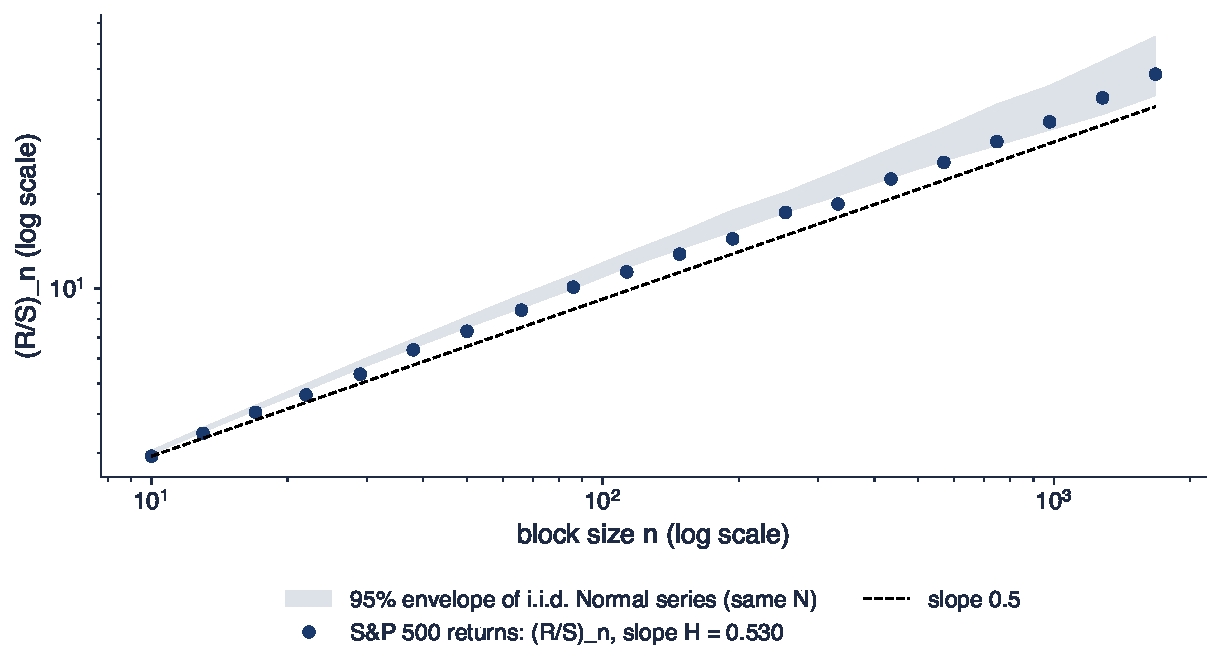
\includegraphics[width=0.96\textwidth,height=0.30\textheight,keepaspectratio]{ch11_sem_b1.pdf}
\end{center}
\vspace{-2mm}
\begin{center}
\scriptsize
\begin{tabular}{lrrrr}
\toprule
 & R/S & DFA & GPH $\hat H = \hat d + 0.5$ & Lo $V(q)$ \\
\midrule
estimate & $0.530$ & $0.488$ & $0.536$ & $1.559$ ($q = 7$) \\
95\% band & $[0.512, 0.575]$ & $[0.456, 0.540]$ & $[0.363, 0.652]$ & $[0.809, 1.862]$ \\
\bottomrule
\end{tabular}
\end{center}
\begin{itemize}
    \item $N = 6\,714$; GPH: $\hat d = 0.036$, SE $0.071$ ($m = 81$), $t = 0.51$; classical $V(0) = 1.379$
    \item Interpretation: no: i.i.d.\ series of this length give R/S $0.544$ on average; every estimate lies inside its band and Lo does not reject short memory
\end{itemize}\sfmquantlet{Ch_11}{SFM_ch11_seminar}
\end{frame}

\begin{frame}{B2: BET and Banca Transilvania [Proposed]}
\itemsize{\footnotesize}
\begin{itemize}
\item \textbf{Question}: does the BET or Banca Transilvania show long memory in returns? Model: B1.
\item \textbf{Inputs}: BET since 2000, TLV since 2010 (without 30--31 May 2016); daily log returns in \%
\item \textbf{Tasks}
\begin{enumerate}
    \item Estimate $H$ with R/S, DFA and GPH for each series.
    \item Compute Lo's $V(q)$ and say whether short memory is rejected at 5\%.
    \item Compute the Monte Carlo band of each estimator for each length.
    \item Interpretation: what could explain the result for the BET?
\end{enumerate}
\item \textbf{Report}: one table and two sentences
\item Notebook: section B2
\end{itemize}
\end{frame}

\ifsolutions
\begin{frame}{B2: Solution [Proposed]}
\itemsize{\footnotesize}
\begin{center}
\scriptsize
\begin{tabular}{lrrrrr}
\toprule
 & $N$ & R/S [band] & DFA [band] & GPH $\hat d$ (SE) & Lo $V(q)$ \\
\midrule
BET & 6\,670 & $0.578$ $[0.507, 0.578]$ & $0.570$ $[0.451, 0.542]$ & $0.166$ ($0.071$) & $1.961$ \\
TLV & 3\,788 & $0.539$ $[0.509, 0.590]$ & $0.473$ $[0.442, 0.551]$ & $-0.063$ ($0.082$) & $1.071$ \\
\bottomrule
\end{tabular}
\end{center}
\begin{itemize}
    \item BET: R/S at the edge of its band, DFA above it, GPH $\hat d$ about 2.33 standard errors from 0, Lo rejects ($1.961 > 1.862$): persistence
    \item TLV: every estimate inside its band; Lo does not reject
    \item Interpretation: thin trading and slow price adjustment in the early years of the BVB (\sfmchlink{https://danpele.github.io/SFM/EN/Courses/chapter7_efficient_markets_random_walk_vr.pdf}{Chapter 7}, variance-ratio tests); the rolling exponents of the lecture show the BET moving towards 0.5
\end{itemize}\sfmquantlet{Ch_11}{SFM_ch11_seminar}
\end{frame}
\fi

\begin{frame}{B3: Long Memory in S\&P 500 Volatility [Solved]}
\itemsize{\footnotesize}
\begin{itemize}
\item \textbf{Question}: do the absolute and the squared S\&P 500 returns have long memory?
\item \textbf{Inputs}: S\&P 500 daily log returns since 2000; $|r_t|$ and $r_t^2$
\item \textbf{Tasks}
\begin{enumerate}
    \item Estimate $d$ with GPH for $m = \lfloor T^{0.5}\rfloor$ and $m = \lfloor T^{0.6}\rfloor$, and $H$ with DFA, for $|r_t|$ and $r_t^2$.
    \item Report the ACF of $|r_t|$ at lags 1, 50 and 250 and the 95\% band $\pm 1.96/\sqrt{T}$.
    \item Shuffle $|r_t|$ at random and repeat the estimates.
    \item Draw the ACF of $|r_t|$ before and after the shuffle.
    \item Interpretation: does long memory in $|r_t|$ contradict the weak form of the EMH?
\end{enumerate}
\item \textbf{Report}: a table, the chart and two sentences
\item Notebook: section B3
\end{itemize}
\end{frame}

\begin{frame}{B3: Solution [Solved]}
\itemsize{\scriptsize}
\begin{center}
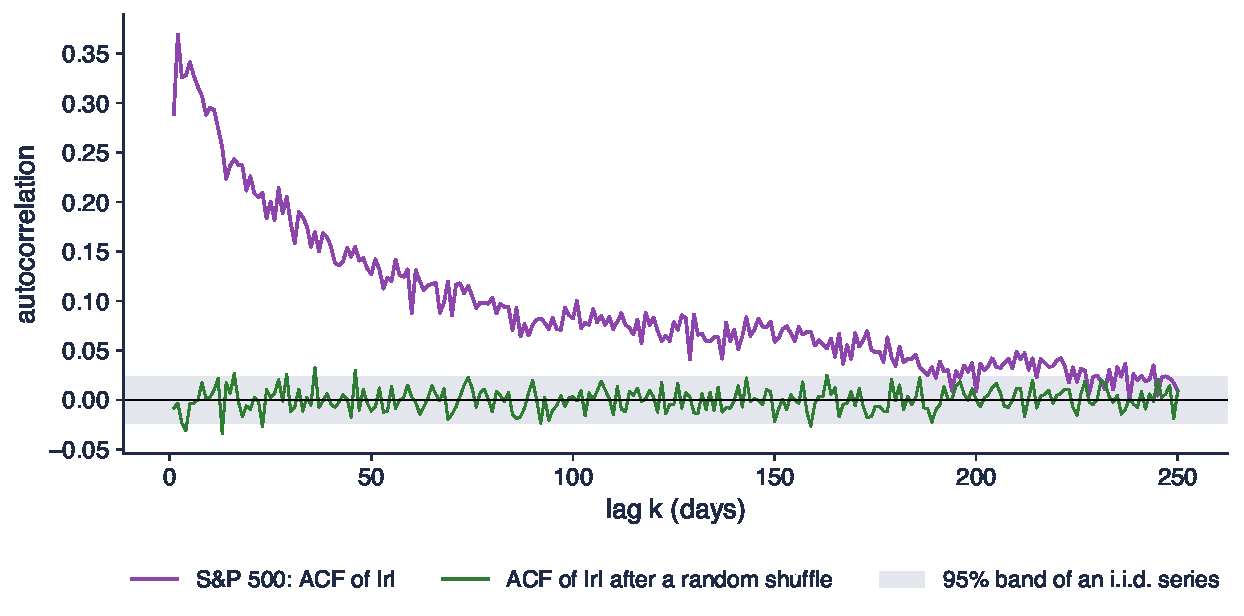
\includegraphics[width=0.96\textwidth,height=0.28\textheight,keepaspectratio]{ch11_sem_b3.pdf}
\end{center}
\vspace{-2mm}
\begin{center}
\scriptsize
\begin{tabular}{lrrrrrr}
\toprule
 & GPH $T^{0.5}$ & GPH $T^{0.6}$ & DFA & $\rho(1)$ & $\rho(50)$ & $\rho(250)$ \\
\midrule
$|r_t|$ & $0.470$ & $0.467$ & $0.953$ & $0.289$ & $0.127$ & $0.009$ \\
$r_t^2$ & $0.326$ & $0.377$ & $0.892$ & $0.313$ & $0.053$ & $-0.010$ \\
$|r_t|$ shuffled & $0.028$ & $-0.001$ & $0.498$ & $-0.008$ & $-0.011$ & $0.009$ \\
\bottomrule
\end{tabular}
\end{center}
\begin{itemize}
    \item $m = 81$ and 197; SE $0.071$ and $0.046$; ACF band $\pm 0.024$; after the shuffle all estimates fall to 0 ($d$) or 0.5 ($H$)
    \item Interpretation: no: the weak form concerns the direction of returns (B1); long memory in $|r_t|$ means predictable risk, which needs a volatility model (\sfmchlink{https://danpele.github.io/SFM/EN/Courses/chapter9_arch_garch_models.pdf}{Chapter 9})
\end{itemize}\sfmquantlet{Ch_11}{SFM_ch11_seminar}
\end{frame}

\begin{frame}{B4: Bitcoin Returns and Volatility [Proposed]}
\itemsize{\footnotesize}
\begin{itemize}
\item \textbf{Question}: does Bitcoin show long memory in returns, in volatility, or in both? Models: B1, B3.
\item \textbf{Inputs}: Bitcoin daily log returns since 2014 (7 days a week)
\item \textbf{Tasks}
\begin{enumerate}
    \item Estimate R/S, DFA, GPH and Lo's $V(q)$ for the returns, with the Monte Carlo bands.
    \item Estimate GPH ($T^{0.5}$, $T^{0.6}$) and DFA for $|r_t|$ and $r_t^2$.
    \item Repeat the volatility estimates after a random shuffle of $|r_t|$.
    \item Interpretation: is Bitcoin closer to the S\&P 500 or to the BET?
\end{enumerate}
\item \textbf{Report}: one table and two sentences
\item Notebook: section B4
\end{itemize}
\end{frame}

\ifsolutions
\begin{frame}{B4: Solution [Proposed]}
\itemsize{\scriptsize}
\begin{center}
\scriptsize
\begin{tabular}{lrrrr}
\toprule
Returns & R/S & DFA & GPH $\hat d$ (SE) & Lo $V(q)$ \\
\midrule
estimate & $0.592$ & $0.561$ & $0.050$ ($0.079$) & $1.547$ \\
95\% band & $[0.508, 0.583]$ & $[0.448, 0.550]$ & $[0.321, 0.659]$ ($\hat H$) & $[0.809, 1.862]$ \\
\bottomrule
\end{tabular}
\end{center}
\begin{center}
\scriptsize
\begin{tabular}{lrrr}
\toprule
Volatility & GPH $T^{0.5}$ & GPH $T^{0.6}$ & DFA \\
\midrule
$|r_t|$ & $0.326$ & $0.355$ & $0.820$ \\
$r_t^2$ & $0.205$ & $0.245$ & $0.664$ \\
$|r_t|$ shuffled & $0.165$ & $0.066$ & $0.527$ \\
\bottomrule
\end{tabular}
\end{center}
\begin{itemize}
    \item Returns: R/S and DFA slightly above their bands, GPH and Lo do not reject: weak evidence, sensitive to the estimator
    \item Volatility: long memory ($\hat d$ around $0.326$), weaker than for the S\&P 500 (B3); gone after the shuffle
    \item Interpretation: between the two: closer to the S\&P 500 in returns, with weaker volatility memory; Lecture 11 shows the rolling estimates
\end{itemize}\sfmquantlet{Ch_11}{SFM_ch11_seminar}
\end{frame}
\fi

\begin{frame}{B5: Rolling Hurst Exponents of the S\&P 500 [Solved]}
\itemsize{\footnotesize}
\begin{itemize}
\item \textbf{Question}: has the memory of S\&P 500 returns changed since 2000?
\item \textbf{Inputs}: S\&P 500 daily log returns since 2000
\item \textbf{Tasks}
\begin{enumerate}
    \item Estimate the DFA exponent on windows of 1000 days moved by 21 days, dated at the last day of each window.
    \item Compute the 95\% Monte Carlo band for $N = 1000$.
    \item Report the minimum and the maximum with their dates, and the share of windows below and above the band.
    \item Draw the rolling exponent with the band.
    \item Interpretation: does a window outside the band prove that the market was inefficient at that time?
\end{enumerate}
\item \textbf{Report}: six numbers, the chart and two sentences
\item Notebook: section B5
\end{itemize}
\end{frame}

\begin{frame}{B5: Solution [Solved]}
\itemsize{\scriptsize}
\begin{center}
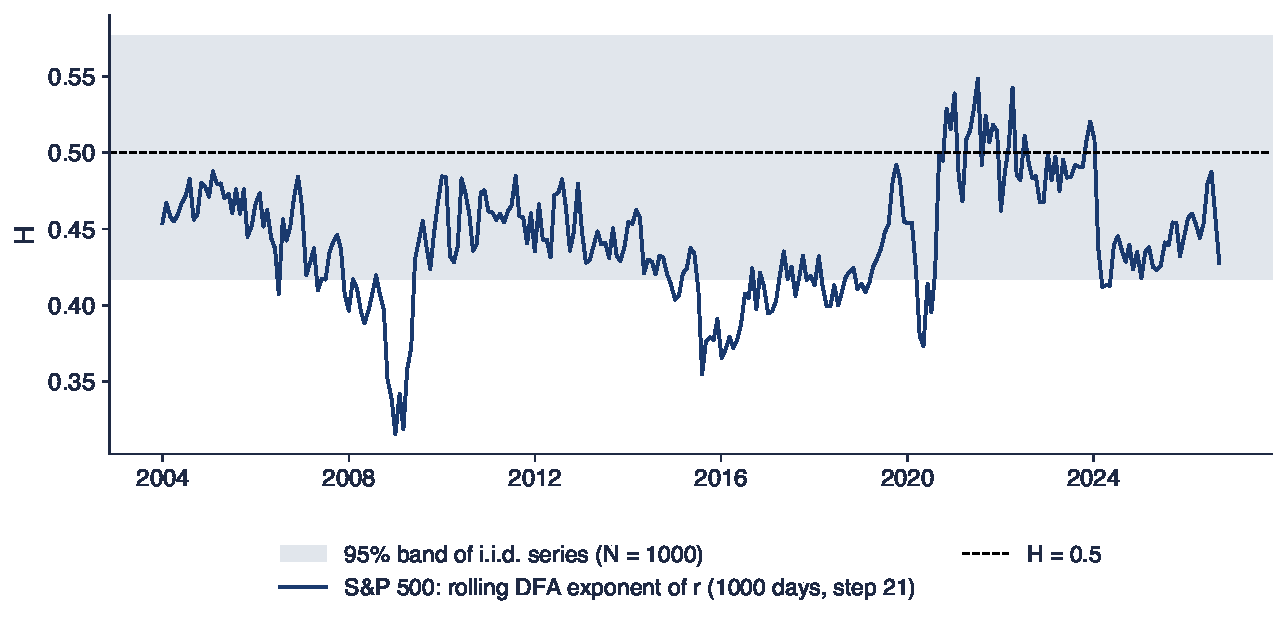
\includegraphics[width=0.96\textwidth,height=0.34\textheight,keepaspectratio]{ch11_sem_b5.pdf}
\end{center}
\vspace{-2mm}
\begin{itemize}
    \item 273 windows from 29 December 2003; band $[0.417, 0.577]$; mean $\hat H = 0.443$
    \item Minimum $0.316$ (31 December 2008), maximum $0.549$ (9 July 2021); 22.3\% of the windows below the band, 0.0\% above
    \item Interpretation: no: by chance about 14 of 273 windows fall outside, and consecutive windows overlap; only long runs count; here the runs are below the band (anti-persistence after 2008 and in 2016), never above
\end{itemize}\sfmquantlet{Ch_11}{SFM_ch11_seminar}
\end{frame}

\begin{frame}{B6: Rolling Exponents of the DAX and of Banca Transilvania [Proposed]}
\itemsize{\footnotesize}
\begin{itemize}
\item \textbf{Question}: does the result of B5 hold for the DAX and for Banca Transilvania? Model: B5.
\item \textbf{Inputs}: DAX since 2000, TLV since 2010; daily log returns in \%
\item \textbf{Tasks}
\begin{enumerate}
    \item Estimate the rolling DFA exponent as in B5.
    \item Report the share of windows below and above the band, and the minimum and maximum with their dates.
    \item Compare the mean exponent in the first and in the last third of the windows.
    \item Interpretation: which market looks more stable over time?
\end{enumerate}
\item \textbf{Report}: one table and two sentences
\item Notebook: section B6
\end{itemize}
\end{frame}

\ifsolutions
\begin{frame}{B6: Solution [Proposed]}
\itemsize{\footnotesize}
\begin{center}
\scriptsize
\begin{tabular}{lrrrrrr}
\toprule
 & windows & below & above & minimum & maximum & first / last third \\
\midrule
DAX & 276 & 4.0\% & 1.8\% & $0.391$ (20 February 2009) & $0.609$ (22 November 2021) & $0.462$ / $0.494$ \\
TLV & 133 & 2.3\% & 0.0\% & $0.400$ (23 July 2024) & $0.559$ (3 September 2014) & $0.512$ / $0.481$ \\
\bottomrule
\end{tabular}
\end{center}
\begin{itemize}
    \item Band for $N = 1000$: $[0.417, 0.577]$
    \item DAX: a few windows outside on both sides, around the 2009 and 2021 extremes; TLV: almost always inside
    \item Interpretation: both are close to 0.5 most of the time; neither shows a lasting departure, unlike the BET in its early years
\end{itemize}\sfmquantlet{Ch_11}{SFM_ch11_seminar}
\end{frame}
\fi


%=============================================================================
\section{Part C: Open Questions and AI Critique}
%=============================================================================

\begin{frame}{C1: Does Market Memory Change in Crises? [Proposed]}
\itemsize{\footnotesize}
\begin{itemize}
\item \textbf{Question}: does the Hurst exponent of returns or of volatility change in a crisis, as the fractal market hypothesis suggests?
\item \textbf{Inputs}: S\&P 500 and BET daily log returns; a calm year (2017) and two crisis years (September 2008--August 2009, February 2020--February 2021); models: B1, B3
\item \textbf{Tasks}
\begin{enumerate}
    \item Estimate the DFA exponent of $r_t$ and of $|r_t|$ and the annualised volatility in each of the three years, for both indices.
    \item Compute the Monte Carlo band for windows of about 250 days.
    \item List three reasons why one crisis year cannot settle the question.
    \item Interpretation: which design would separate a change of memory from a change of volatility?
\end{enumerate}
\item \textbf{Report}: a table and a plan for a project
\item Notebook: section C1
\end{itemize}
\end{frame}

\ifsolutions
\begin{frame}{C1: Reference Analysis [Proposed]}
\itemsize{\footnotesize}
\begin{center}
\scriptsize
\begin{tabular}{llrrrr}
\toprule
Index & period & $N$ & DFA $r_t$ & DFA $|r_t|$ & volatility \\
\midrule
S\&P 500 & calm 2017 & 250 & $0.42$ & $0.51$ & 6.7\% \\
S\&P 500 & crisis 2008--2009 & 252 & $0.43$ & $0.76$ & 45.2\% \\
S\&P 500 & crisis 2020--2021 & 251 & $0.69$ & $1.02$ & 34.9\% \\
BET & calm 2017 & 248 & $0.58$ & $0.68$ & 10.5\% \\
BET & crisis 2008--2009 & 249 & $0.44$ & $0.67$ & 51.4\% \\
BET & crisis 2020--2021 & 249 & $0.76$ & $0.87$ & 25.2\% \\
\bottomrule
\end{tabular}
\end{center}
\begin{itemize}
    \item Band for $N = 250$: $[0.33, 0.66]$; only the 2020--2021 returns of both indices lie above it
    \item Reasons: one year gives a wide band; the volatility level changes the estimate of $|r_t|$; the rebound after March 2020 is a trend inside the window
    \item Design: standardise $r_t$ by a GARCH volatility (\sfmchlink{https://danpele.github.io/SFM/EN/Courses/chapter9_arch_garch_models.pdf}{Chapter 9}) before estimating; use many crises and markets, event windows, and a GARCH-based band; compare with the wavelet approach of \refKrisB
\end{itemize}\sfmquantlet{Ch_11}{SFM_ch11_seminar}
\end{frame}
\fi

\begin{frame}{C2: Audit an AI Answer [Proposed]}
\itemsize{\scriptsize}
\begin{itemize}
    \item A student asked an AI assistant to interpret long-memory estimates for the S\&P 500 (daily, since 2000). The answer:
    \item \aiprompt{(a) R/S gives H = 0.530 for the returns: above 0.5, so returns have long memory and trends can be exploited.}
    \item \aiprompt{(b) H = 0.530 means a 53\% probability that tomorrow has the same sign as today.}
    \item \aiprompt{(c) GPH gives d = 0.470 for |r|, so H = d - 0.5 = -0.030: absolute returns are anti-persistent.}
    \item \aiprompt{(d) Long memory in |r| contradicts the weak form of the EMH.}
    \item \aiprompt{(e) Lo's modified statistic V = 1.56 lies inside [0.809, 1.862], so short memory is not rejected at 5\%.}
    \item \aiprompt{(f) For more precision, use all T/2 = 3357 frequencies in the GPH regression.}
    \item Tasks
    \begin{itemize}
        \item 1. For each statement, say whether it is correct; if not, give the correct statement and, where possible, the correct number from the notebook (section C2).
        \item 2. Report: a list of six verdicts with one line of justification each.
    \end{itemize}
\end{itemize}
\end{frame}

\ifsolutions
\begin{frame}{C2: Solution [Proposed]}
\itemsize{\footnotesize}
\begin{itemize}
    \item (a) Wrong: i.i.d.\ series of this length give R/S $0.544$ on average, band up to $0.575$; DFA gives $0.488$: no evidence of long memory (B1)
    \item (b) Wrong: $H$ is a scaling exponent, not a probability
    \item (c) Wrong: $H = d + 0.5 = 0.970$: strong persistence of volatility
    \item (d) Wrong: the weak form concerns the direction of returns; predictable volatility is compatible with it (B3, \sfmchlink{https://danpele.github.io/SFM/EN/Courses/chapter9_arch_garch_models.pdf}{Chapter 9})
    \item (e) Correct
    \item (f) Wrong: high frequencies carry the short-run dynamics and bias $\hat d$; GPH needs $m/T \to 0$; report $m = T^{0.5}$ and $T^{0.6}$
\end{itemize}\sfmquantlet{Ch_11}{SFM_ch11_seminar}
\end{frame}
\fi


%=============================================================================
\section{Wrap-Up}
%=============================================================================

\begin{frame}{What You Should Take from Today}
\itemsize{\small}
\begin{itemize}
    \item R/S, DFA and GPH estimate the same $H$ in different ways; report several, each with a Monte Carlo band for the same $N$
    \item $d = H - 0.5$; $H$ is a scaling exponent, not a probability
    \item Returns of large markets: no long memory; volatility: long memory everywhere; the shuffle test locates it in the order of the days
    \item Rolling estimates: read long runs outside the band, not single windows
    \item An AI answer is a draft: check the band, the conversion between $d$ and $H$, and the bandwidth
\end{itemize}
\end{frame}

\begin{frame}{After the Seminar}
\itemsize{\small}
\begin{itemize}
    \item Lecture 11 develops each topic of today: the FMH, self-similarity, fBm and ARFIMA, the estimators, spurious memory, rolling exponents, risk scaling
    \item Try the [Proposed] tasks in the notebook; the solutions are discussed in class
    \item C1 can grow into a team project: GARCH-standardised returns, many crises, a GARCH-based band
    \item Reading: \refFHH, Ch.~14; \refLo; \refWeron
\end{itemize}
\end{frame}


%=============================================================================
\section{References}
%=============================================================================

\begin{frame}{References}
\itemsize{\tiny}
\begin{itemize}
    \item Anis, A.A., Lloyd, E.H. (1976). \href{https://doi.org/10.1093/biomet/63.1.111}{The expected value of the adjusted rescaled Hurst range of independent normal summands}. \textit{Biometrika}, 63(1), 111--116.
    \item Diebold, F.X., Inoue, A. (2001). \href{https://doi.org/10.1016/S0304-4076(01)00073-2}{Long memory and regime switching}. \textit{Journal of Econometrics}, 105(1), 131--159.
    \item Ding, Z., Granger, C.W.J., Engle, R.F. (1993). \href{https://doi.org/10.1016/0927-5398(93)90006-D}{A long memory property of stock market returns and a new model}. \textit{Journal of Empirical Finance}, 1(1), 83--106.
    \item Franke, J., Härdle, W.K., Hafner, C.M. (2019). \href{https://doi.org/10.1007/978-3-030-13751-9}{\textit{Statistics of Financial Markets: An Introduction}}, 5th ed. Springer.
    \item Geweke, J., Porter-Hudak, S. (1983). \href{https://doi.org/10.1111/j.1467-9892.1983.tb00371.x}{The estimation and application of long memory time series models}. \textit{Journal of Time Series Analysis}, 4(4), 221--238.
    \item Hosking, J.R.M. (1981). \href{https://doi.org/10.1093/biomet/68.1.165}{Fractional differencing}. \textit{Biometrika}, 68(1), 165--176.
    \item Hurst, H.E. (1951). \href{https://doi.org/10.1061/TACEAT.0006518}{Long-term storage capacity of reservoirs}. \textit{Transactions of the American Society of Civil Engineers}, 116(1), 770--799.
    \item Kristoufek, L. (2013). \href{https://doi.org/10.1038/srep02857}{Fractal markets hypothesis and the global financial crisis: wavelet power evidence}. \textit{Scientific Reports}, 3, 2857.
    \item Lo, A.W. (1991). \href{https://doi.org/10.2307/2938368}{Long-term memory in stock market prices}. \textit{Econometrica}, 59(5), 1279--1313.
    \item Mandelbrot, B.B., Van Ness, J.W. (1968). \href{https://doi.org/10.1137/1010093}{Fractional Brownian motions, fractional noises and applications}. \textit{SIAM Review}, 10(4), 422--437.
    \item Peng, C.-K., Buldyrev, S.V., Havlin, S., Simons, M., Stanley, H.E., Goldberger, A.L. (1994). \href{https://doi.org/10.1103/PhysRevE.49.1685}{Mosaic organization of DNA nucleotides}. \textit{Physical Review E}, 49(2), 1685--1689.
    \item Peters, E.E. (1994). \href{https://www.wiley.com/en-us/Fractal+Market+Analysis\%3A+Applying+Chaos+Theory+to+Investment+and+Economics-p-9780471585244}{\textit{Fractal Market Analysis: Applying Chaos Theory to Investment and Economics}}. Wiley.
    \item Weron, R. (2002). \href{https://doi.org/10.1016/S0378-4371(02)00961-5}{Estimating long-range dependence: finite sample properties and confidence intervals}. \textit{Physica A}, 312(1--2), 285--299.
\end{itemize}
\end{frame}

\end{document}
